% Auriga theme
% https://github.com/anishathalye/auriga

\documentclass[14pt,aspectratio=169]{beamer}
\usepackage{pgfpages}
\usepackage{amsmath}
\usepackage{fancyvrb}
\usepackage{tikz}
\usetikzlibrary{arrows.meta, positioning, quotes}
\usepackage{pgfplots}

% \ifnotes
% \setbeamertemplate{note page}[plain]
% \setbeameroption{show notes on second screen=right}
% \fi

\usetheme{auriga}
\usecolortheme{auriga}

% define some colors for a consistent theme across slides
\definecolor{red}{RGB}{181, 23, 0}
\definecolor{blue}{RGB}{0, 118, 186}
\definecolor{gray}{RGB}{146, 146, 146}

\title{Universidad Nacional de La Plata (UNLP) \\ Maestría en Finanzas
  Públicas Provinciales y Municipales \\ La Politica de las Finanzas
  Públicas}
\subtitle{Clase 3}
\author{\underline{Sebastian Freille} \inst{1}}
\institute[IEF (FCE-UNC)]{\inst{1} Instituto de Economía y Finanzas (FCE-UNC)}
\date{}



\AtBeginSection[]{
    \begin{frame}
    \vfill
    \centering
    \begin{beamercolorbox}[sep=8pt,center,shadow=true,rounded=true]{title}
        \usebeamerfont{title}\insertsectionhead\par%
    \end{beamercolorbox}
    \vfill
    \end{frame}
}


\begin{document}
\maketitle



\section{Decisiones colectivas en democracia representativa: Partidos
  políticos y competencia electoral}


\begin{frame}\frametitle{TVM y democracia representativa}
\begin{itemize}
\item El teorema del votante mediano (TVM) a pesar de ser muy
  intuitivo se cumple baja condiciones muy estrictas
  \item En las democracias modernas, no se eligen directamente las
    políticas sino que ciudadanos votan a representantes y estos
    eligen las políticas $\longrightarrow$ ¿problema?
    \item Esto se conoce como democracia representativa. Problemas
      princiales $\longrightarrow$ 1) elegir un candidato de un
      conjunto; 2) implementar la política anunciada
\end{itemize}
\end{frame}



\begin{frame}\frametitle{Competencia electoral}
\begin{itemize}
\item Elemento central de las democracias representativas es la
  \textbf{competencia electoral} $\longrightarrow$ en el caso de 2
  (dos) partidos (coaliciones de partidos) puede verse como un juego de suma
  cero simultáneo entre 2 (dos) jugadores.
  \item Los individuos no eligen las políticas directamente --eligen
    partidos políticos que anuncian la política a implementar
    \item Versión simple e idealizada de democracia represenativa
\end{itemize}
\end{frame}


\begin{frame}\frametitle{Competencia diferenciada: ¿espacial?}
\begin{itemize}
\item En 1929, Hotelling observó que las empresas competidoras solían
  imitar la calidad de los bienes y la
  localización. ¿Por qué teniendo un enorme
  mercado geográfico para localizarse se establecen tan cerca (por qué
  imitaban calidad del producto)?
\item Ejemplo $\longrightarrow$ vendedores de helados en una
  playa. ¿Donde deben localizarse a lo largo de una playa de 1km si
  los individuos están distribuidos uniformemente?
  \item Esto se observa en la vida real
    $\longrightarrow$ heladeras en supermercados; negocios en una
    misma cuadra/zona.
\end{itemize}
\end{frame}


\begin{frame}
\frametitle{Competencia electoral: Downs}
\begin{itemize} 
\item Preguntas relevantes: \medskip
\begin{itemize} \itemsep 10pt
\item ¿Qué determina el número de partidos políticos y las propuestas de política elegidas?
\item ¿Cómo afecta el sistema electoral el resultado de una elección y las preferencias de los votantes?
\end{itemize}
\item Modelo fundacional $\longrightarrow$ Downs: cada candidato (de un total ``n'') elige una propuesta de política; cada ciudadano tiene preferencias acerca de esas propuestas de política y vota por los candidatos en función de aquellas.
\end{itemize}
\end{frame}


\begin{frame}\frametitle{Competencia electoral: Downs (cont.)}
  \begin{itemize}
  \item Supuestos:
    \begin{itemize}
      \item Cada partido político busca ganar para obtener ingreso,
        prestigio y poder que viene con el cargo;
      \item El partido ganador tiene control completo de sus acciones
      hasta la próxima eleccion
      \item Poderes económicos del gobierno ilimitados
        --dentro del marco democrático. El único límite es político
        $\longrightarrow$ no puede restringir la libertad política
        \item Cada agente en el modelo --votante, partido o coalicion-
          es racional en todo momento 
        \end{itemize}
\end{itemize}      
  \end{frame}



  \begin{frame}\frametitle{Competencia electoral: Downs (cont.)}
    \begin{itemize}
\item Basado en esto desarrolló el \textbf{modelo espacial de
  competencia electoral}. 
\item Continuo
  ideológico unidimensional $[0,100]$, entre economía completamente
  socializada (0) y economía totalmente privada (100).
\item Supuesto $\longrightarrow$ todo puede
  reducirse a la ideología; unidimensional.
  \end{itemize}
  \end{frame}
  


 \begin{frame}\frametitle{Competencia electoral: Downs (cont.)}
   \begin{block}{Hipótesis central}
Los partidos políticos en una democracia formulan la política
estrictamente como un medio para obtener votos (y ganar
elecciones). Para Downs los partidos políticos no son mas que comerciantes
vendiendo ``políticas'' por ``votos''.  
          \end{block}
\end{frame}



\begin{frame}
\frametitle{Competencia electoral: Downs (cont.)}
\begin{itemize}
\item Candidatos son jugadores y la propuesta de política
  es un numero (identifica \textit{posición}). Primero, candidatos eligen las posiciones. Segundo, los ciudadanos votan
\item Otros supuestos: \medskip
\begin{itemize} \itemsep 10pt
\item El único objetivo de cada candidato es ganar
\item Ningún candidato tiene afinidad ideológica
\item Cada candidato prefiere ganar antes que empatar --el resultado se decide por sorteo, y empatar antes que perder.
\item \textit{Continuo} de votantes, cada uno con una posición favorita.
\item La distribucioń de las posiciones favoritas es arbitraria.
\end{itemize}
\end{itemize}
\end{frame}


\begin{frame}
\frametitle{Competencia electoral: Downs (cont.)}
\begin{itemize} 
\item \textit{posición mediana, $m$} $\longrightarrow$ tiene la propiedad de que exactamente la mitad de las posiciones favoritas de los votantes son como máximo $m$ y la mitad de las posiciones favoritas de los votantes son como mínimo $m$ 
\item La distancia entre cualquier posición y la posición favorita de un votante es una medida de la intensidad del desagrado $\longrightarrow$ a mayor distancia, mayor su desagrado
\item Ej $\longrightarrow$ para cualquier valor $k$, un votante cuya posición favorita $x^{*}$ es indiferente entre entre las posiciones $x^{*}-k$ y $x^{*}+k$
\end{itemize}
\end{frame}


\begin{frame}
\frametitle{Competencia electoral: Downs (cont.)}
% \begin{center}
% \begin{figure}
% \psset{unit=0.75cm}
% \begin{pspicture}(0,0)(6,4)
% \psline[linewidth=0.005,linecolor=black]{}(0,3.5)(6,3.5)
% \psline[linewidth=0.025](0,0)(2.99,3.49)
% \psline[linewidth=0.025](3,3.49)(6,0)
% \rput(3,3.9){$x^{*}$}
% \rput(1,3.9){$x^{*}-k$}
% \rput(5,3.9){$x^{*}+k$}
% \psline[linewidth=0.005]{->}(5.6,3.2)(5.9,3.2)
% \rput(5.35,3.2){$x$}
% \psline[linewidth=0.005,linestyle=dashed](1,1.2)(1,3.5)
% \psline[linewidth=0.005,linestyle=dashed](5,1.2)(5,3.5)
% \psline[linewidth=0.005,linestyle=dashed](1,1.2)(5,1.2)
% \end{pspicture} \bigskip
% \caption{Utilidad de un votante con posición favorita $x^{*}$ como función de $x$}
% \end{figure}
% \end{center}

\begin{figure}[htbp]\vspace{-0.5cm}
  \centering
  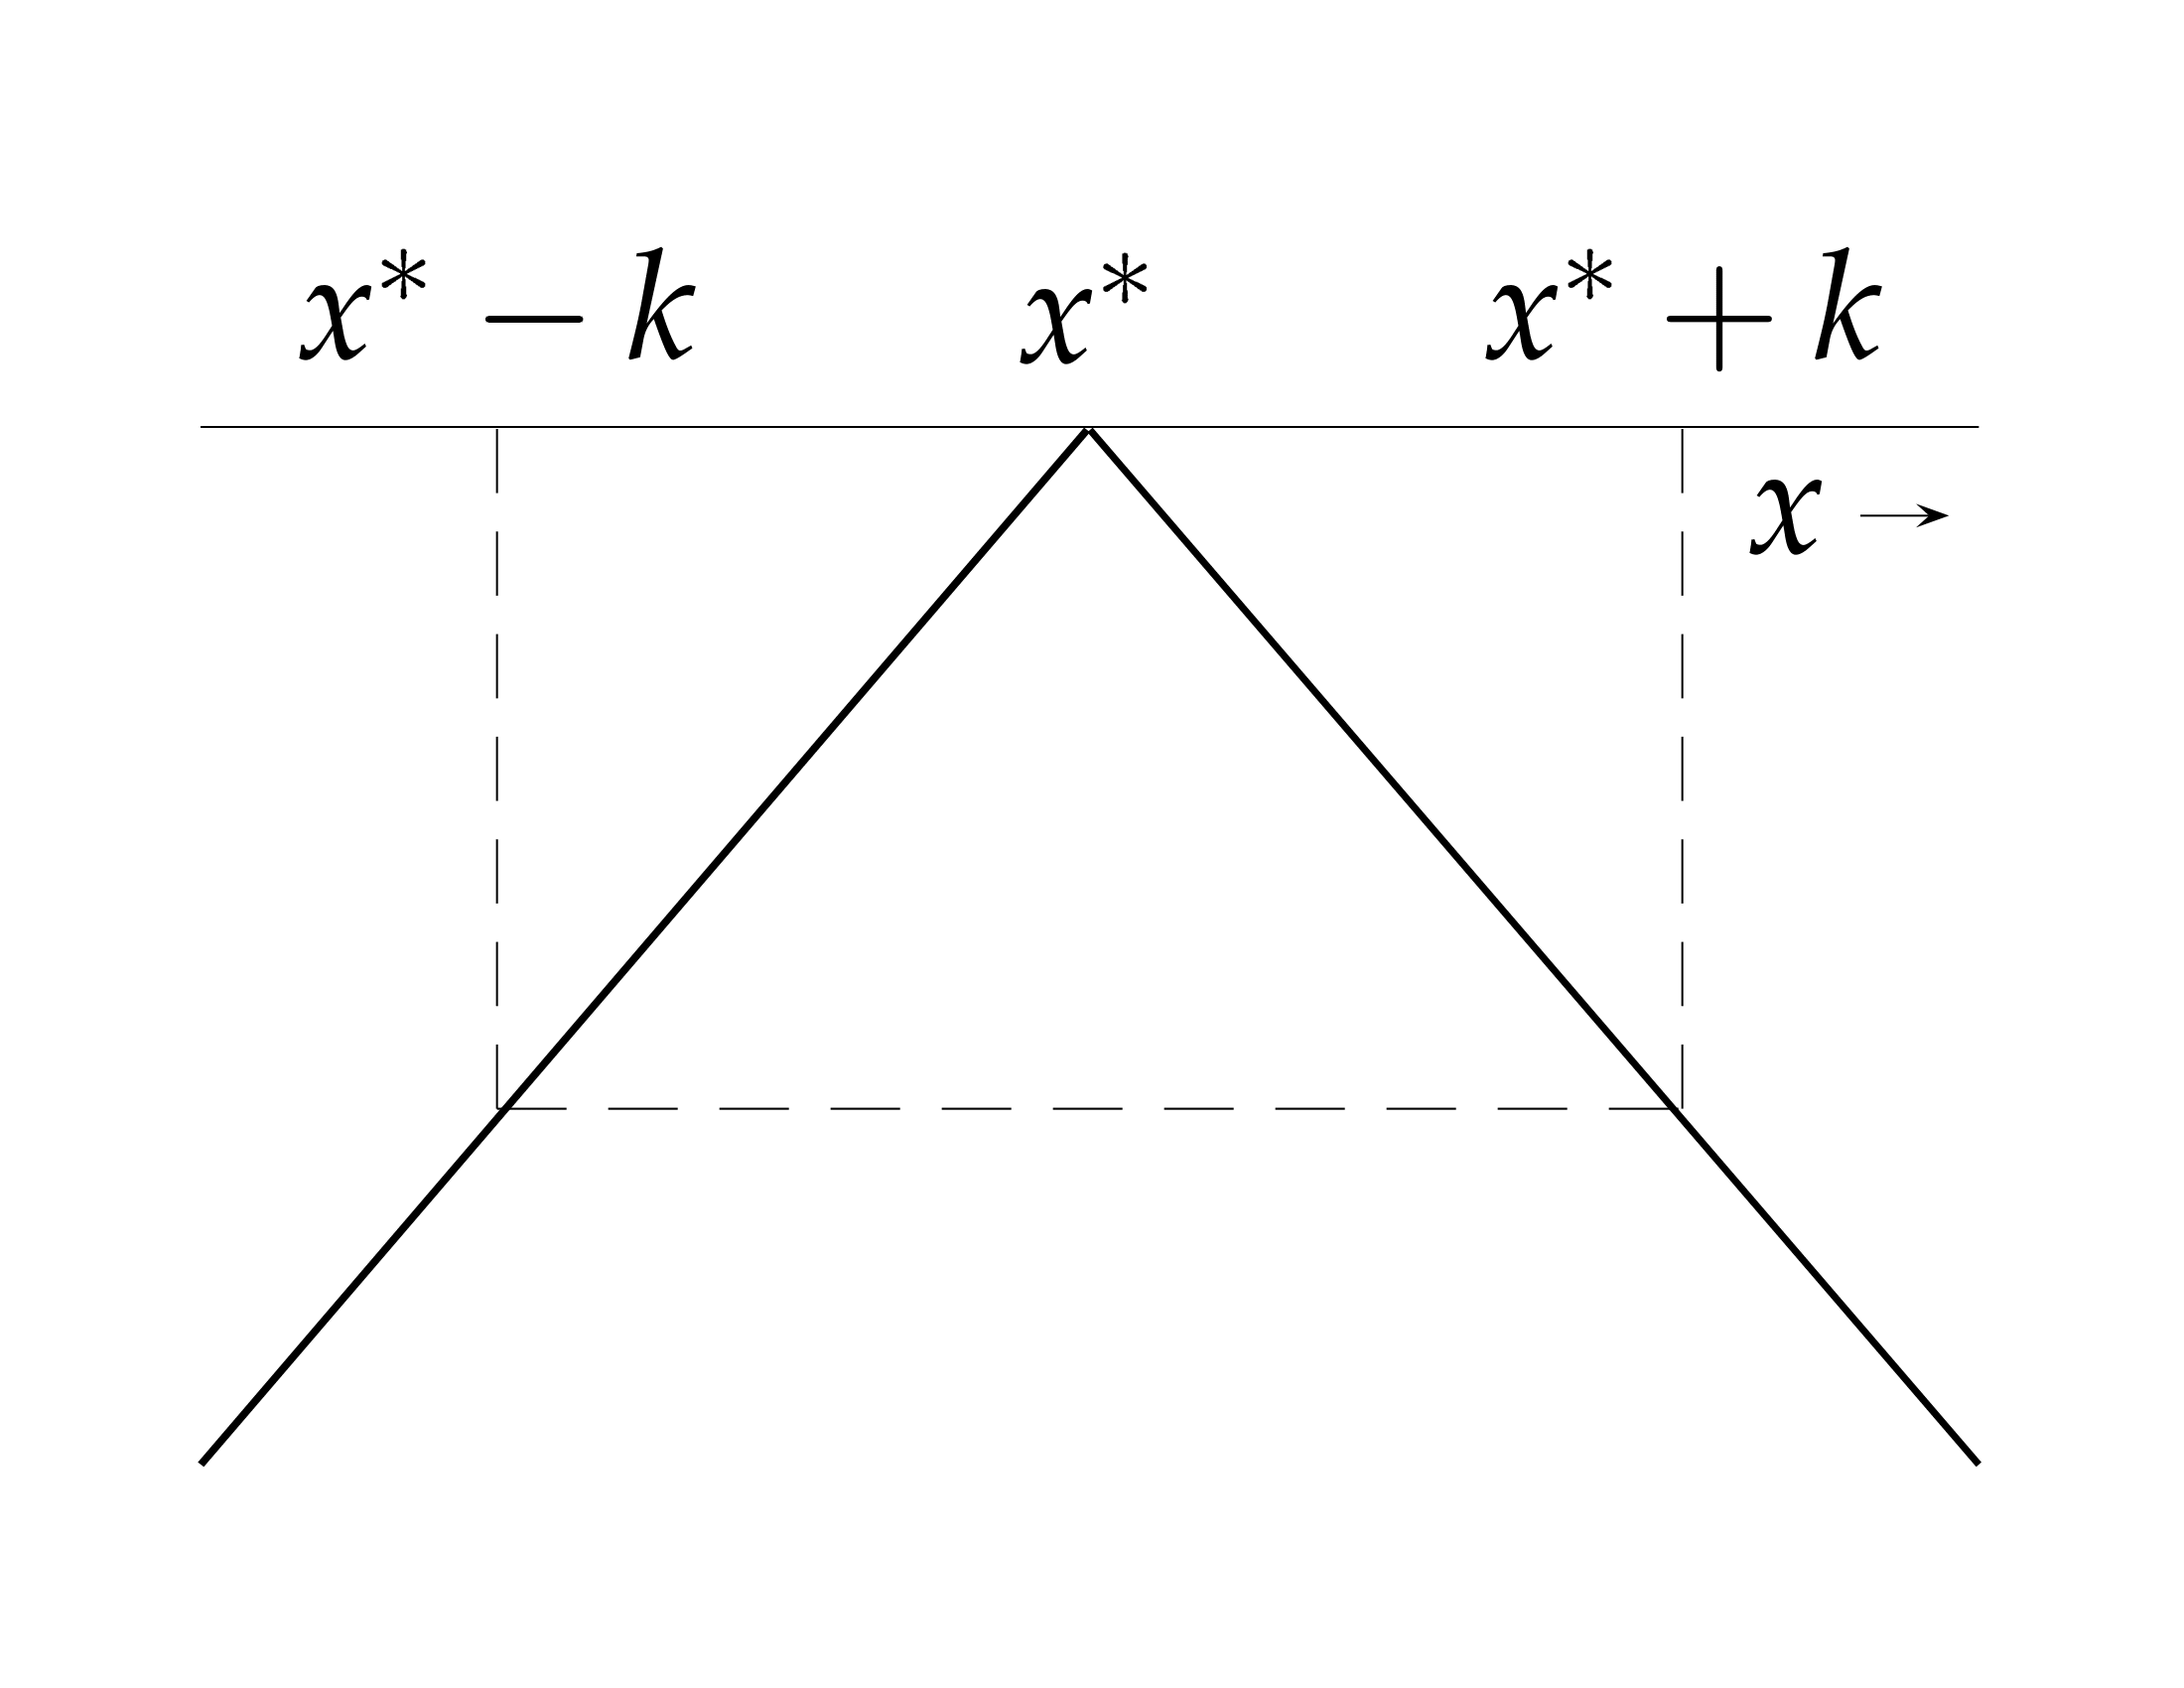
\includegraphics[scale=0.20]{tvm2}\vspace{-1cm}
  \caption{Utilidad de un individuo con posición ideal x* como funcion
    de x}
  \label{fig:3}
\end{figure}
\begin{itemize}\itemsep 10pt
\item Cada candidato atrae los votos de ciudadanos cuyas posiciones favoritas están más cerca de su posición que las de cualquier otro candidato
\end{itemize}
\end{frame}

% \begin{frame}
% \frametitle{Una aplicación: competencia electoral (cont.)}
% \begin{center}
%   \url{run:/animation.gif}
% \end{center}
% \end{frame}


\begin{frame}
\frametitle{Competencia electoral: Downs (cont.)}
% \begin{center}
% \begin{figure}
% \begin{pspicture}(0,0)(8,1)
% \psline[linecolor=black]{|-|}(0,0.5)(8,0.5)
% \psline[linecolor=black]{-}(2.5,0.4)(2.5,0.6)
% \psline[linecolor=black]{-}(5.25,0.4)(5.25,0.6)
% \psdot(1,0.5)
% \psdot(4,0.5)
% \psdot(6.5,0.5)
% \rput(1,0.9){$x_{1}$}
% \rput(4,0.9){$x_{2}$}
% \rput(6.6,0.9){$x_{3}$}
% \rput(0,0.9){$x_{min}$}
% \rput(8,0.9){$x_{max}$}
% \rput(2.5,0.9){\footnotesize{$\frac{1}{2}(x_{1}+x_{2})$}}
% \rput(5.25,0.9){\footnotesize{$\frac{1}{2}(x_{2}+x_{3})$}}
% \rput(1.25,0.1){\scriptsize{votos para 1}}
% \rput(4,0.1){\scriptsize{votos para 2}}
% \rput(6.5,0.1){\scriptsize{votos para 3}}
% \psline[linewidth=0.005]{<-}(0.05,0.1)(0.5,0.1)
% \psline[linewidth=0.005]{->}(2,0.1)(2.45,0.1)
% \psline[linewidth=0.005]{<-}(2.55,0.1)(3.25,0.1)
% \psline[linewidth=0.005]{->}(4.75,0.1)(5.2,0.1)
% \psline[linewidth=0.005]{<-}(5.3,0.1)(5.75,0.1)
% \psline[linewidth=0.005]{->}(7.3,0.1)(7.95,0.1)
% \psline[linecolor=black,linewidth=0.005]{-}(2.5,0.0)(2.5,0.2)
% \psline[linecolor=black,linewidth=0.005]{-}(5.25,0.0)(5.25,0.2)
% \end{pspicture} \bigskip
% \caption{Modelo de competencia electoral de Hoteling-Downs}
% \end{figure}
% \end{center}
\begin{figure}[htbp] \vspace{-2cm}
  \centering
  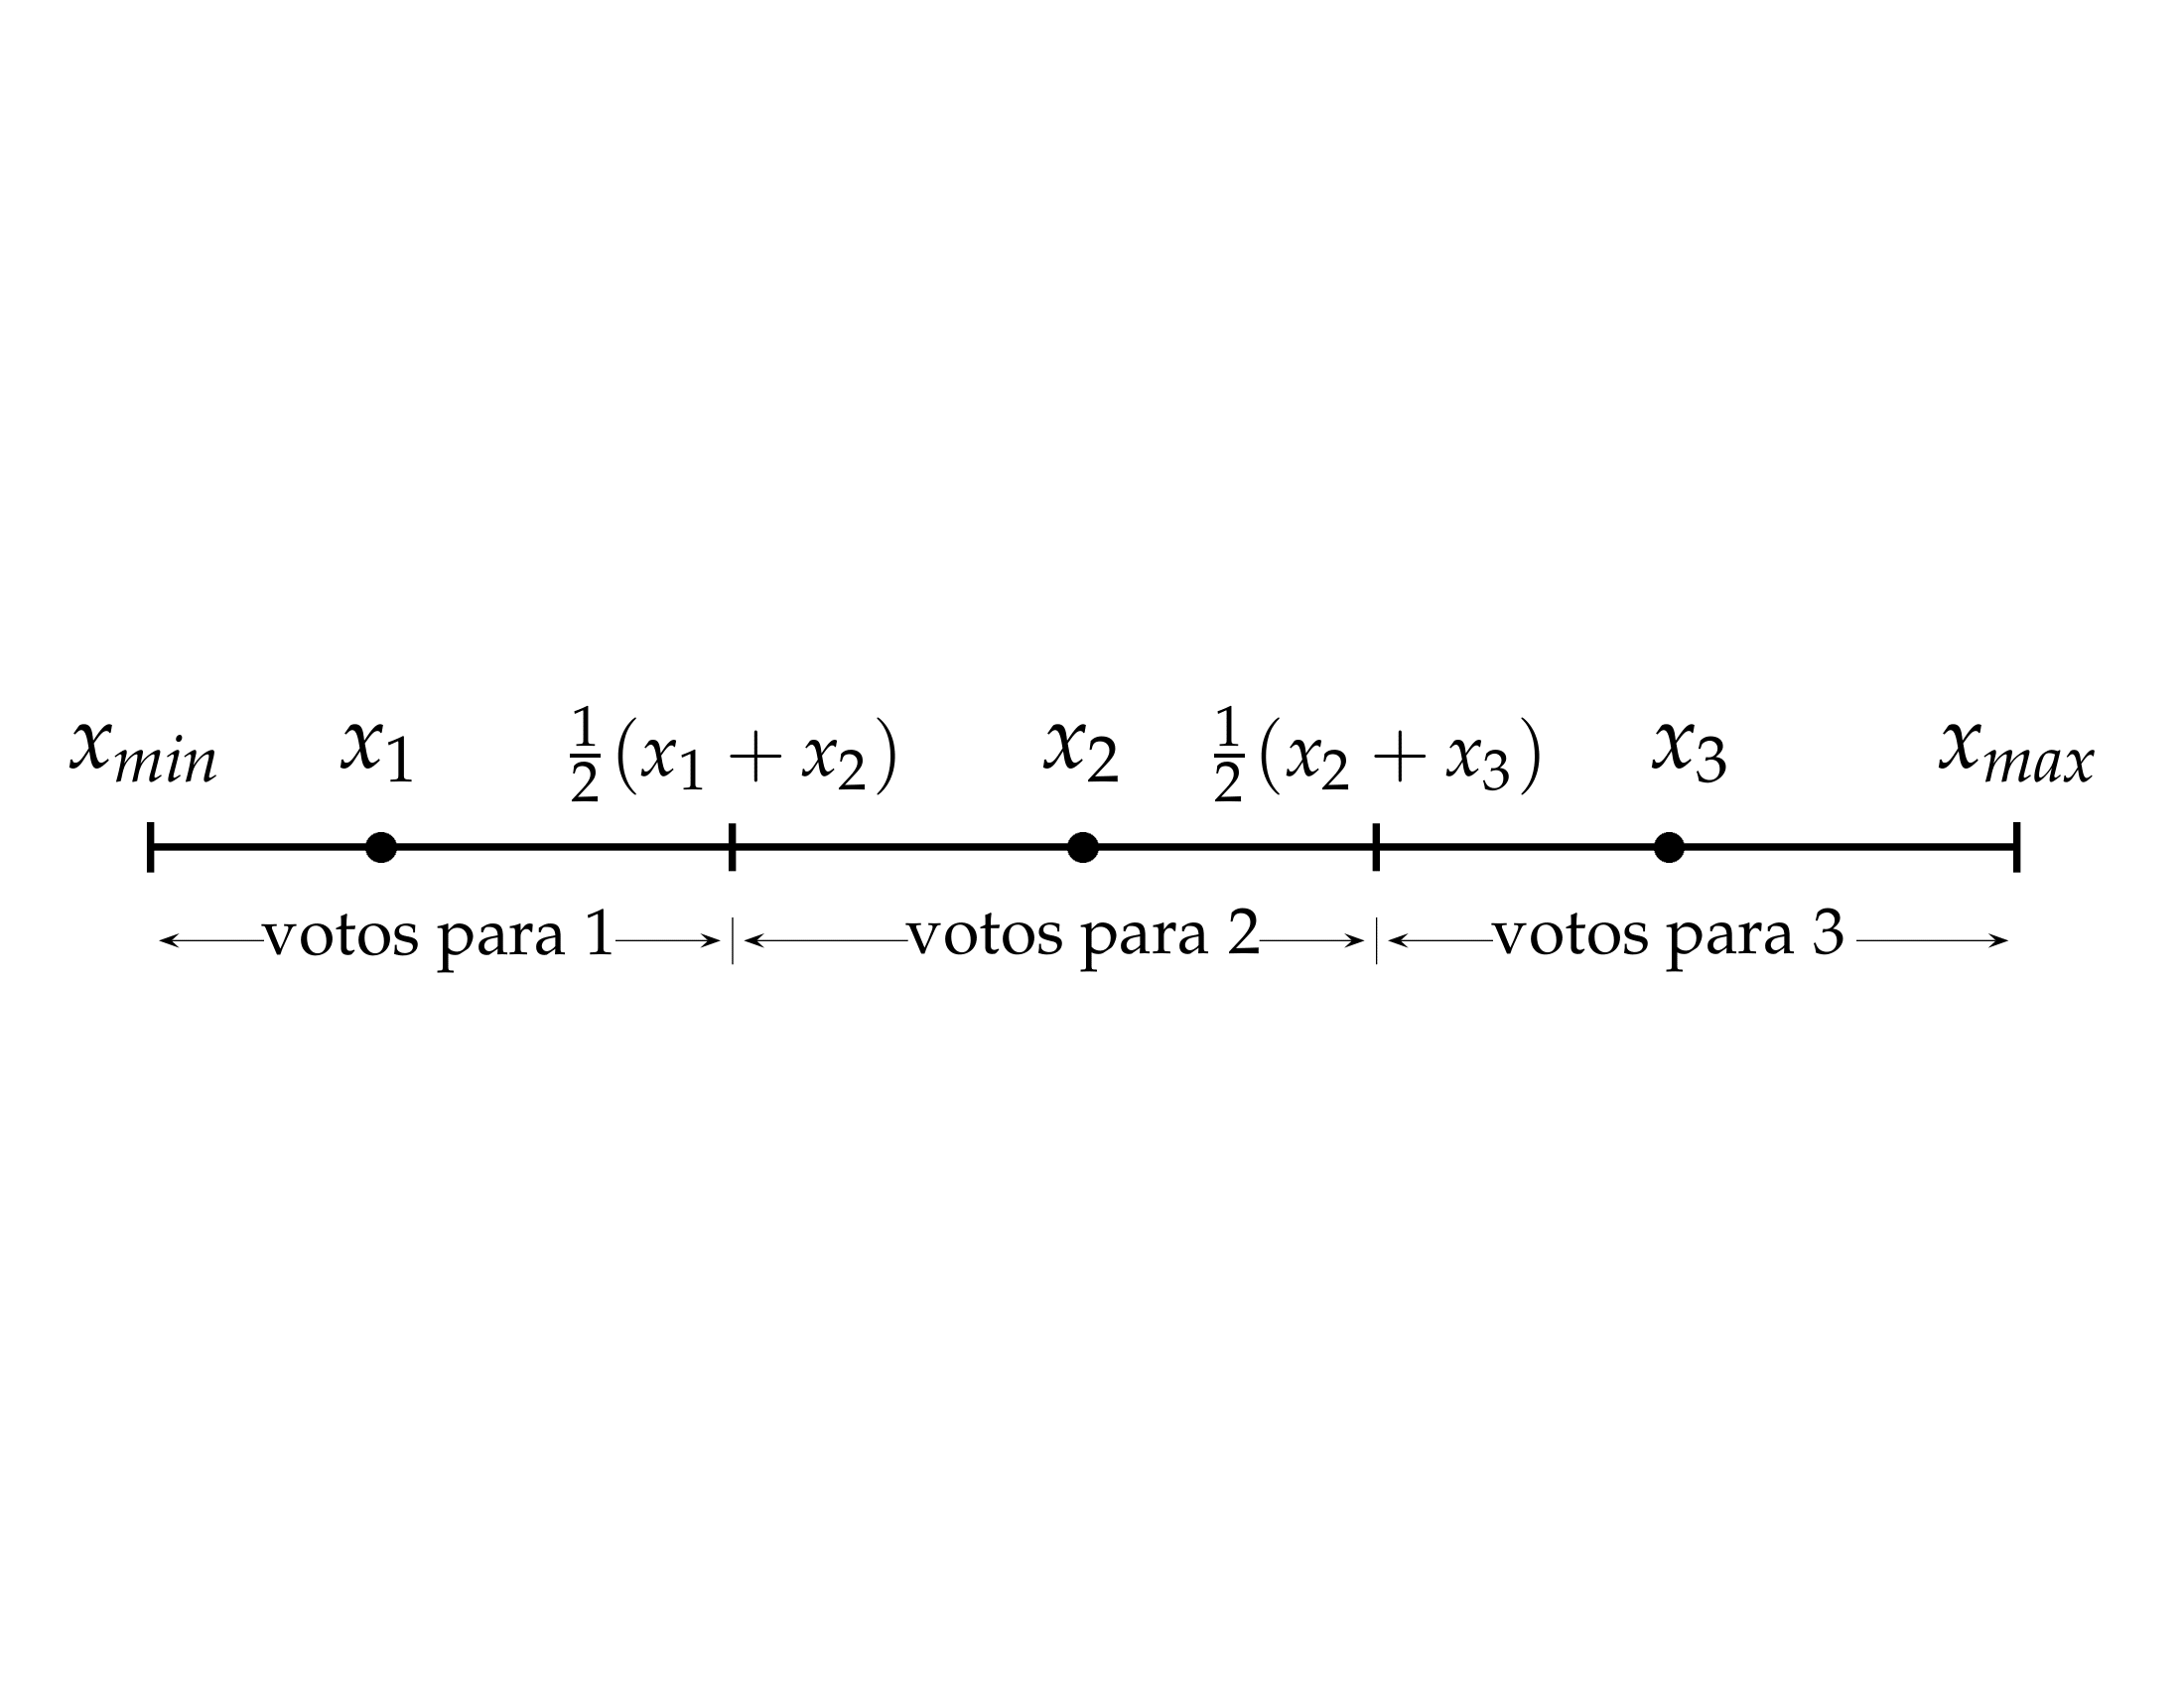
\includegraphics[scale=0.26]{tvm3} \vspace{-3cm}
  \caption{Modelo de competencia electoral de Hoteling-Downs}
  \label{fig:3}
\end{figure}
\vspace{-0.5cm}
\begin{itemize}\itemsep 10pt
\item 3 candidatos: $1$, $2$ y $3$ $\longrightarrow$ 3 posiciones:
  $x_{1}$, $x_{2}$, $x_{3}$ [$x_{1}<x_{2}<x_{3}$]
\item Ciudadanos cuyas posición favorita es $\frac{1}{2}(x_{1}+x_{2})$
  dividen sus votos por igual entre $x_{1}$ y $x_{2}$.
\item Jugadores son los
  \textbf{candidatos}, acciones  el conjunto de
  \textbf{posiciones posibles} y los \textit{payoffs} son $n\succ k
  \succ 0$
\end{itemize}
\end{frame}


\begin{frame}
\frametitle{Competencia electoral: Downs (cont.)}
\begin{itemize}
\item Caso más simple $\longrightarrow$ dos candidatos
\item Fijamos la posición elegida $x_{2}$ del candidato 2 y
  consideramos la mejor respuesta del candidato 1. \medskip
\end{itemize}
% \begin{center}
% \begin{figure}
% \begin{pspicture}(0,0)(8,1)
% \psline[linecolor=black]{|-|}(0,0.5)(8,0.5)
% \psline[linecolor=black]{-}(3,0.4)(3,0.6)
% \psline[linecolor=black]{-}(4,0.4)(4,0.6)
% \psdot(1,0.5)
% \psdot(5,0.5)
% \rput(1,0.9){$x_{2}$}
% \rput(5,0.9){$x_{1}$}
% \rput(4,0.9){$m$}
% \rput(0,0.9){$x_{min}$}
% \rput(8,0.9){$x_{max}$}
% \rput(3,0.9){\footnotesize{$\frac{1}{2}(x_{1}+x_{2})$}}
% \rput(1.5,0.1){\scriptsize{votos para 2}}
% \rput(5.5,0.1){\scriptsize{votos para 1}}
% \psline[linewidth=0.005]{<-}(0.05,0.1)(0.75,0.1)
% \psline[linewidth=0.005]{->}(2.25,0.1)(2.95,0.1)
% \psline[linewidth=0.005]{<-}(3.05,0.1)(4.75,0.1)
% \psline[linewidth=0.005]{->}(6.25,0.1)(7.95,0.1)
% \psline[linecolor=black,linewidth=0.005]{-}(3,0.0)(3,0.2)
% \end{pspicture} \bigskip
% \caption{Equilibrio de Hoteling-Downs con dos candidatos}
% \end{figure}
% \end{center}
\begin{figure}[htbp] \vspace{-2cm}
  \centering
  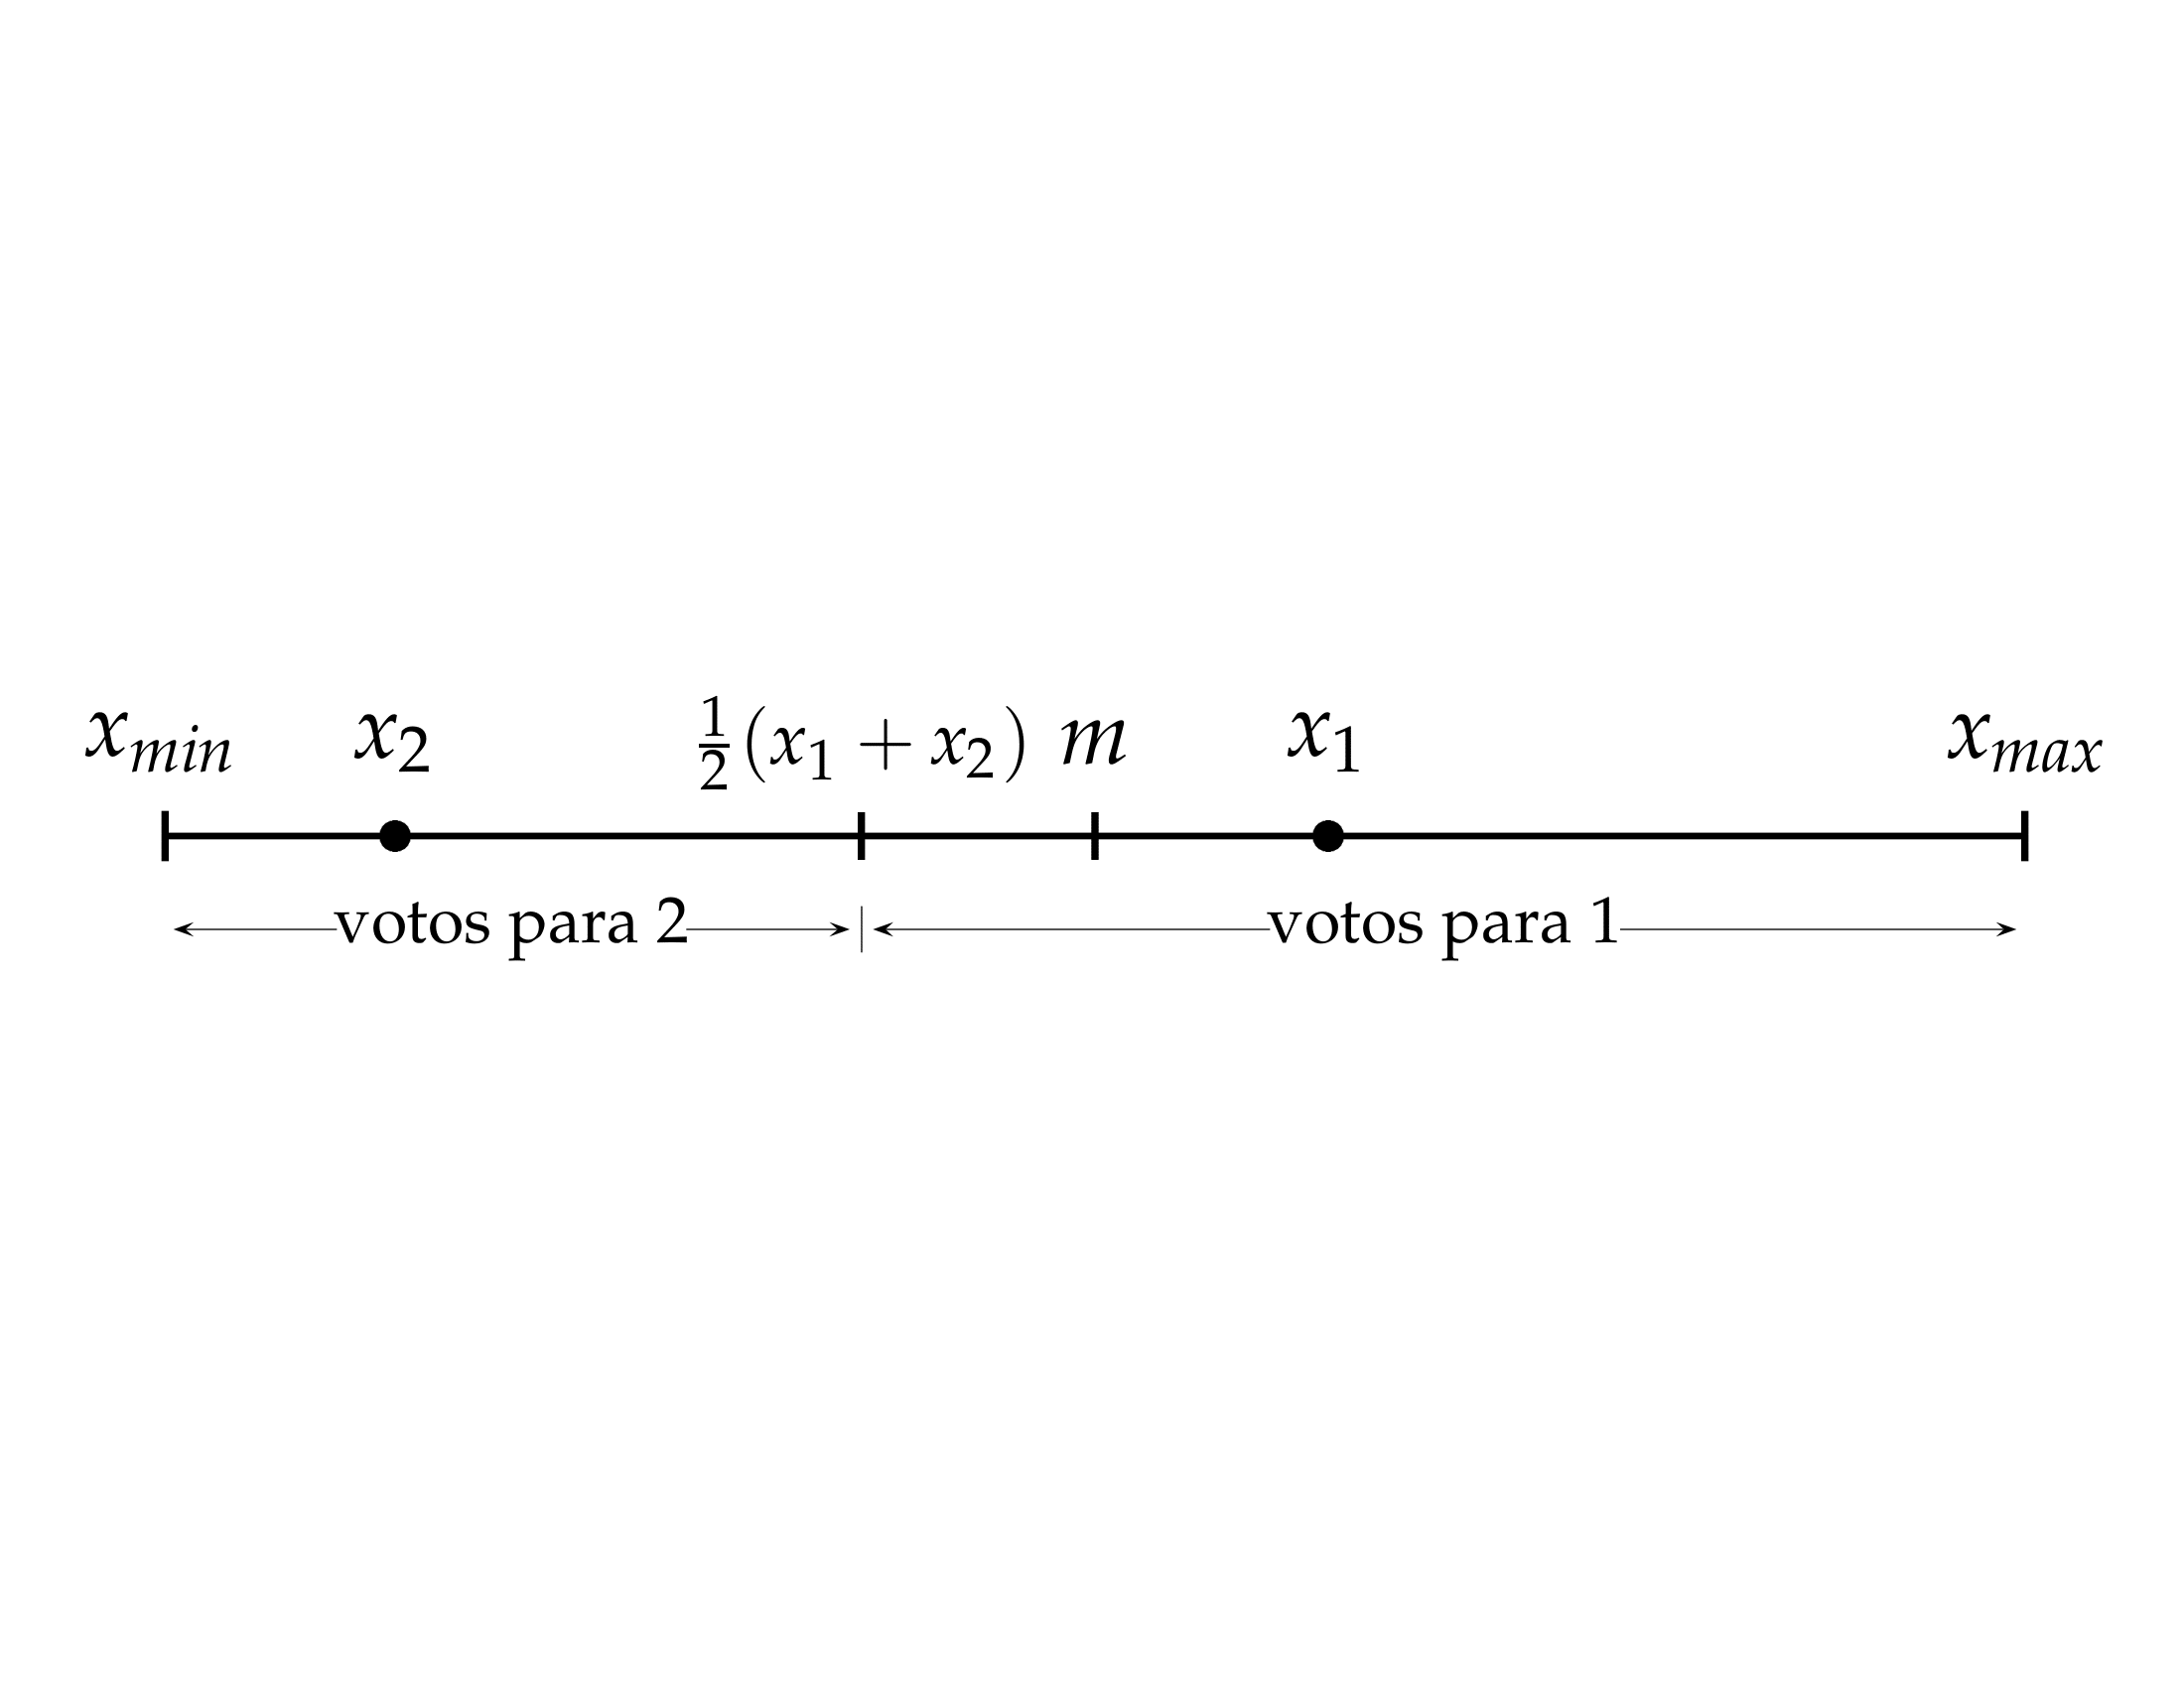
\includegraphics[scale=0.25]{tvm4} \vspace{-3cm}
  \caption{Equilibrio de Hoteling-Downs con dos candidatos}
  \label{fig:3}
\end{figure}

\begin{itemize}\itemsep 10pt
\item Suponga que $x_{2}<m$ $\longrightarrow$ su mejor respuesta es el
  conjunto entre $x_{2}$ y $2m-x_{2}$ [¿Por qué?]
\end{itemize}
\end{frame}


\begin{frame}
\frametitle{Competencia electoral: Downs (cont.)}
\begin{itemize}
\item Suponga ahora que $x_{2}>m$ $\longrightarrow$ su mejor respuesta es el
  conjunto entre $2m-x_{2}$ y $x_{2}$ [¿Por qué?]
\item Finalmente, considere el caso en que $x_{2}=m$ $\longrightarrow$
  la única mejor respuesta del candidato 1 es elegir \textit{la misma
    posición!} que el candidato 2. Cualquier posición diferente de $m$
  y el candidato perderá; si escoge $m$, empata el primer puesto.
\item La \textit{funcion de mejor respuesta} del candidato 1:
\end{itemize} \medskip
\[B_{1}(x_{2}) = \left\{
\begin{array}{l l}
  \left\{x_{1}:x_{2}<x_{1}<2m-x_{2}\right\} & \quad \mbox{if
    $x_{2}<m$}\\
\left\{m\right\} & \quad \mbox{if $x_{2}=m$}\\
\left\{x_{1}:2m-x_{2}<x_{1}<x_{2}\right\} & \quad \mbox{if
    $x_{2}>m$} \\
\end{array} \right. \]
\end{frame}

\begin{frame}\frametitle{Competencia electoral: Downs (cont.)}
  \begin{itemize}
\item Downs no \textit{requiere} que partidos siempre vayan al centro
  \item Si los votantes se distribuyen uniformemente a lo largo del
    eje ``x'' y el partido A originalmente se ubica en A (25) y y el
    partido B se ubica en B (75), a ambos les conviene moverse hacia
    50.
    \item Si la distribución de votantes cambia, los partidos: a)
      tiende a ir a los extremos
      (figura 2); b) tenderan a posicionarse
      alrededor de nucleos de votantes (figura 3) 
    \end{itemize}
  \end{frame}


  \begin{frame}\frametitle{Competencia electoral: Downs (cont.)}
  \begin{figure}[htbp] \vspace{-1cm}
  \centering
  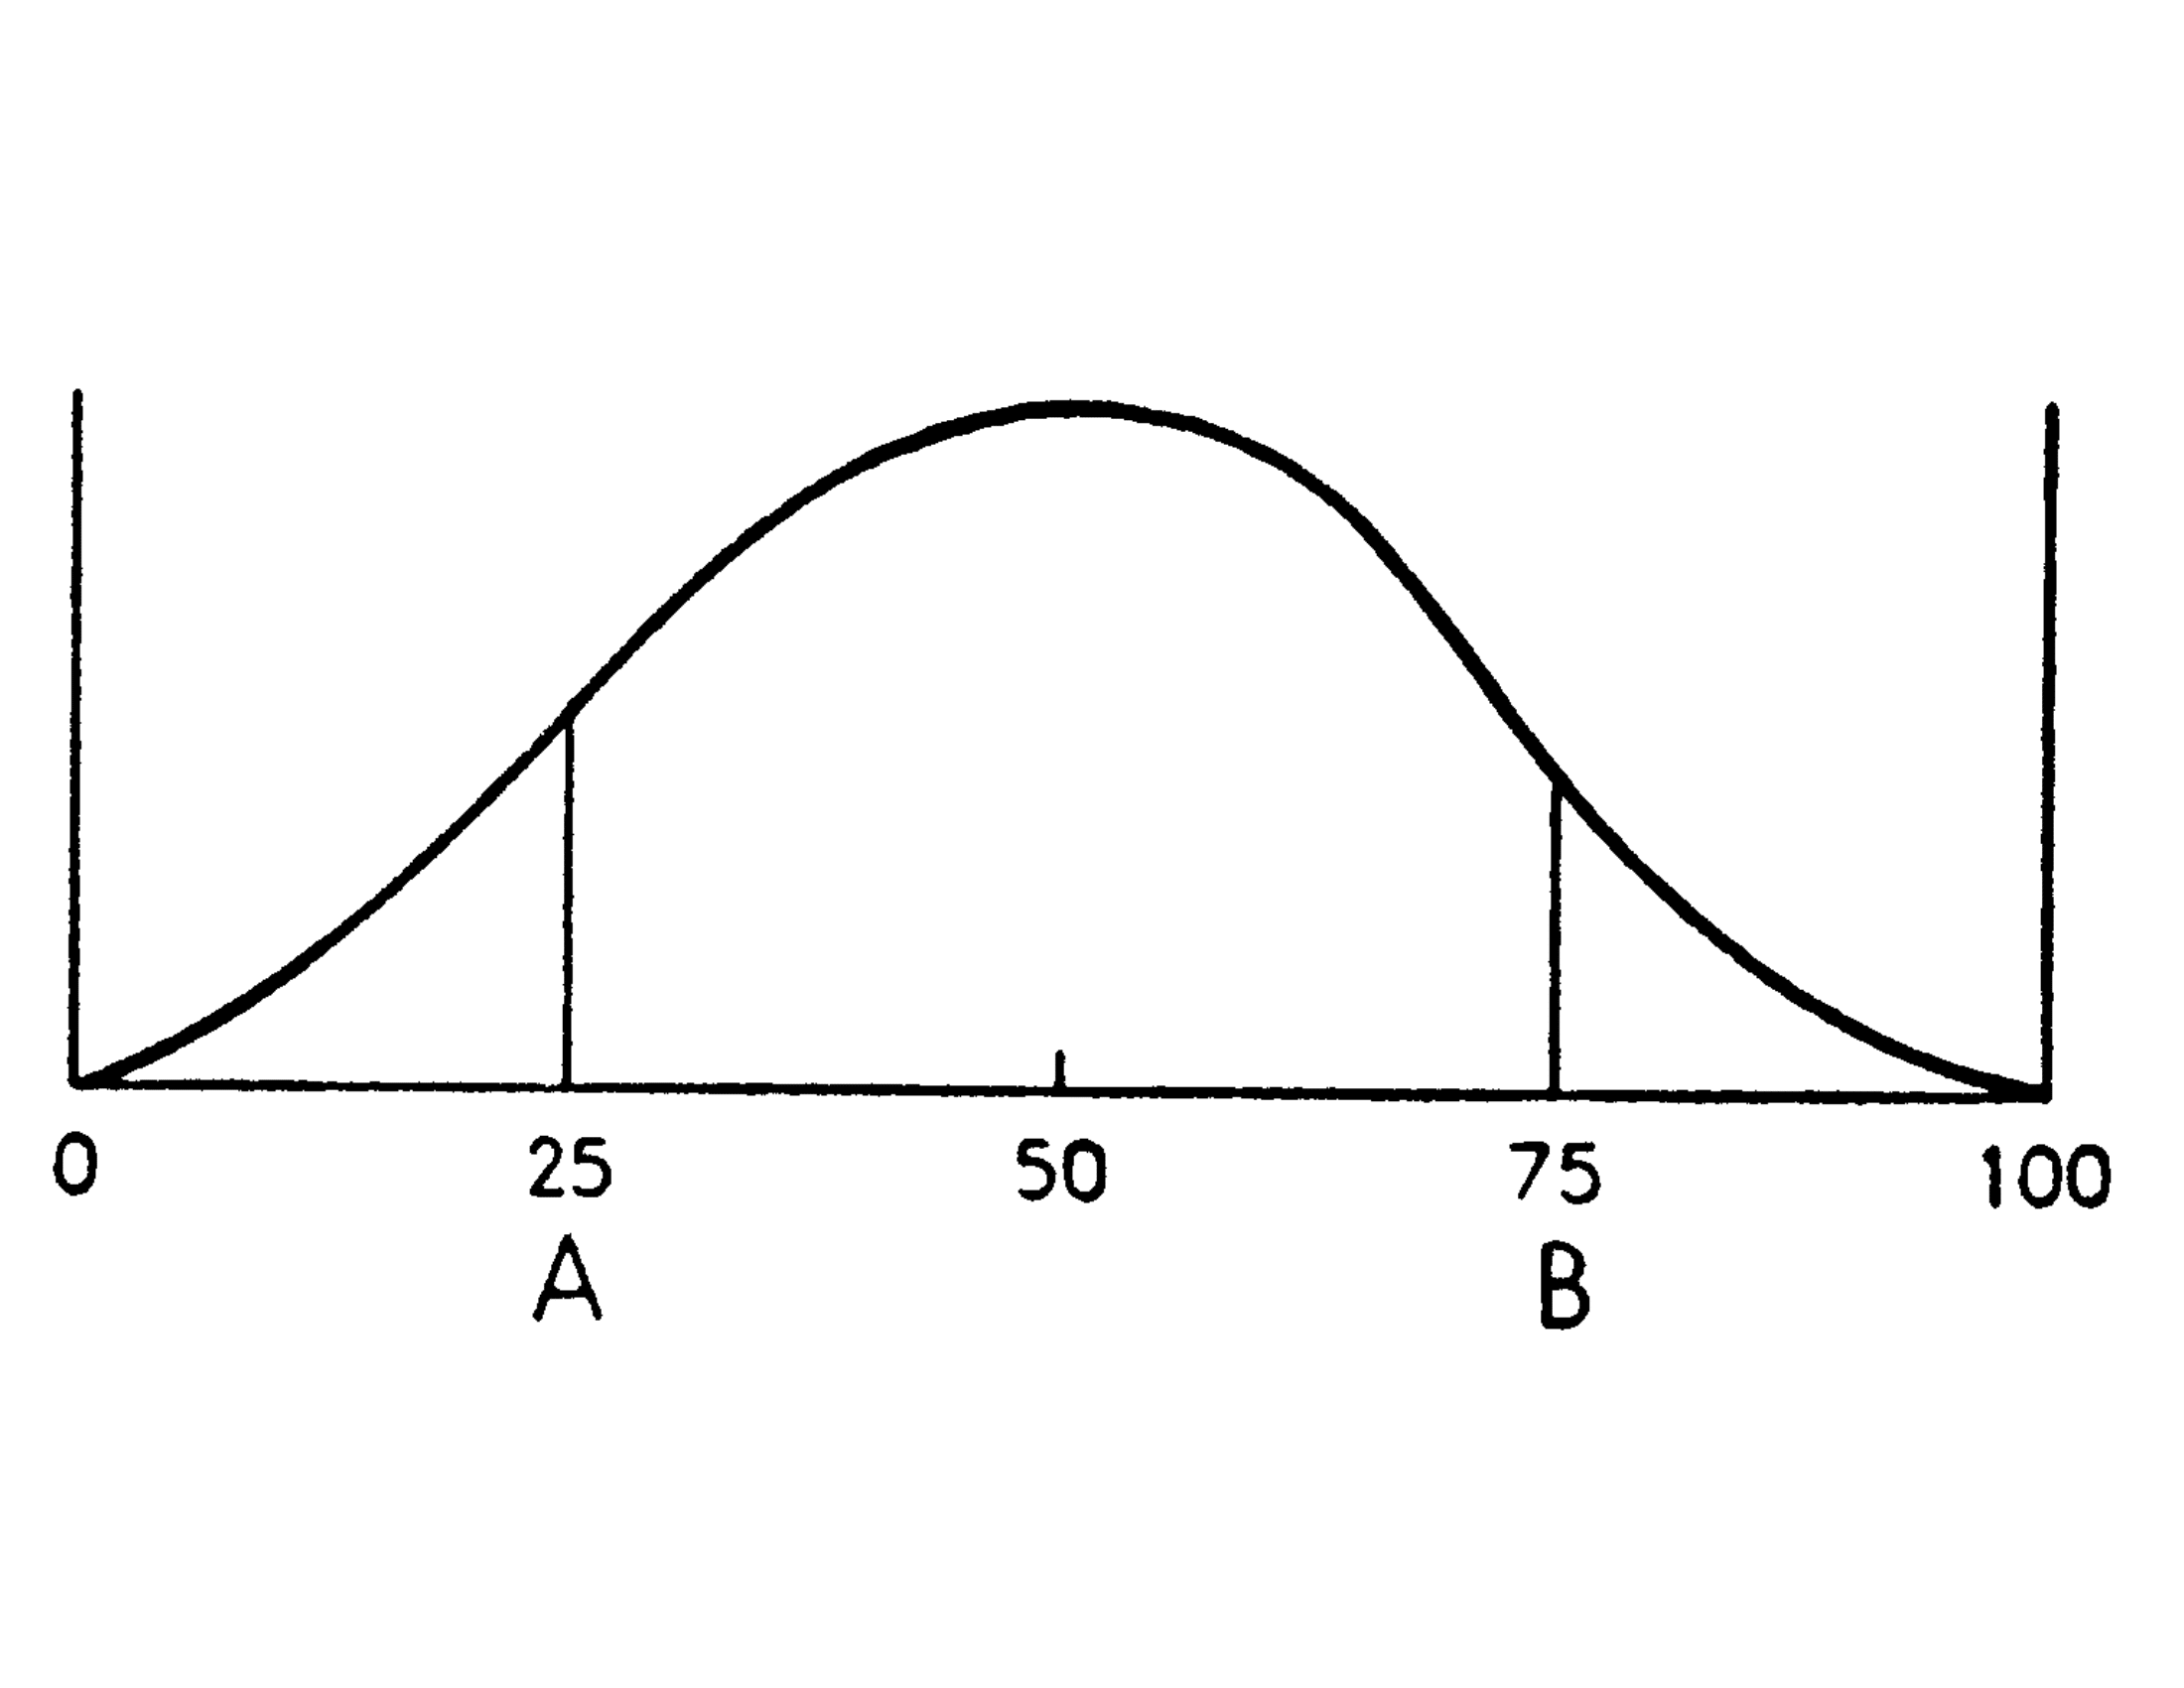
\includegraphics[scale=0.3]{downs5} \vspace{-1cm}
  \caption{Distribución de votantes - Electorado distribución normal}
  \label{fig:3}
\end{figure}
    \end{frame}


     \begin{frame}\frametitle{Competencia electoral: Downs (cont.)}
  \begin{figure}[htbp] \vspace{-1cm}
  \centering
  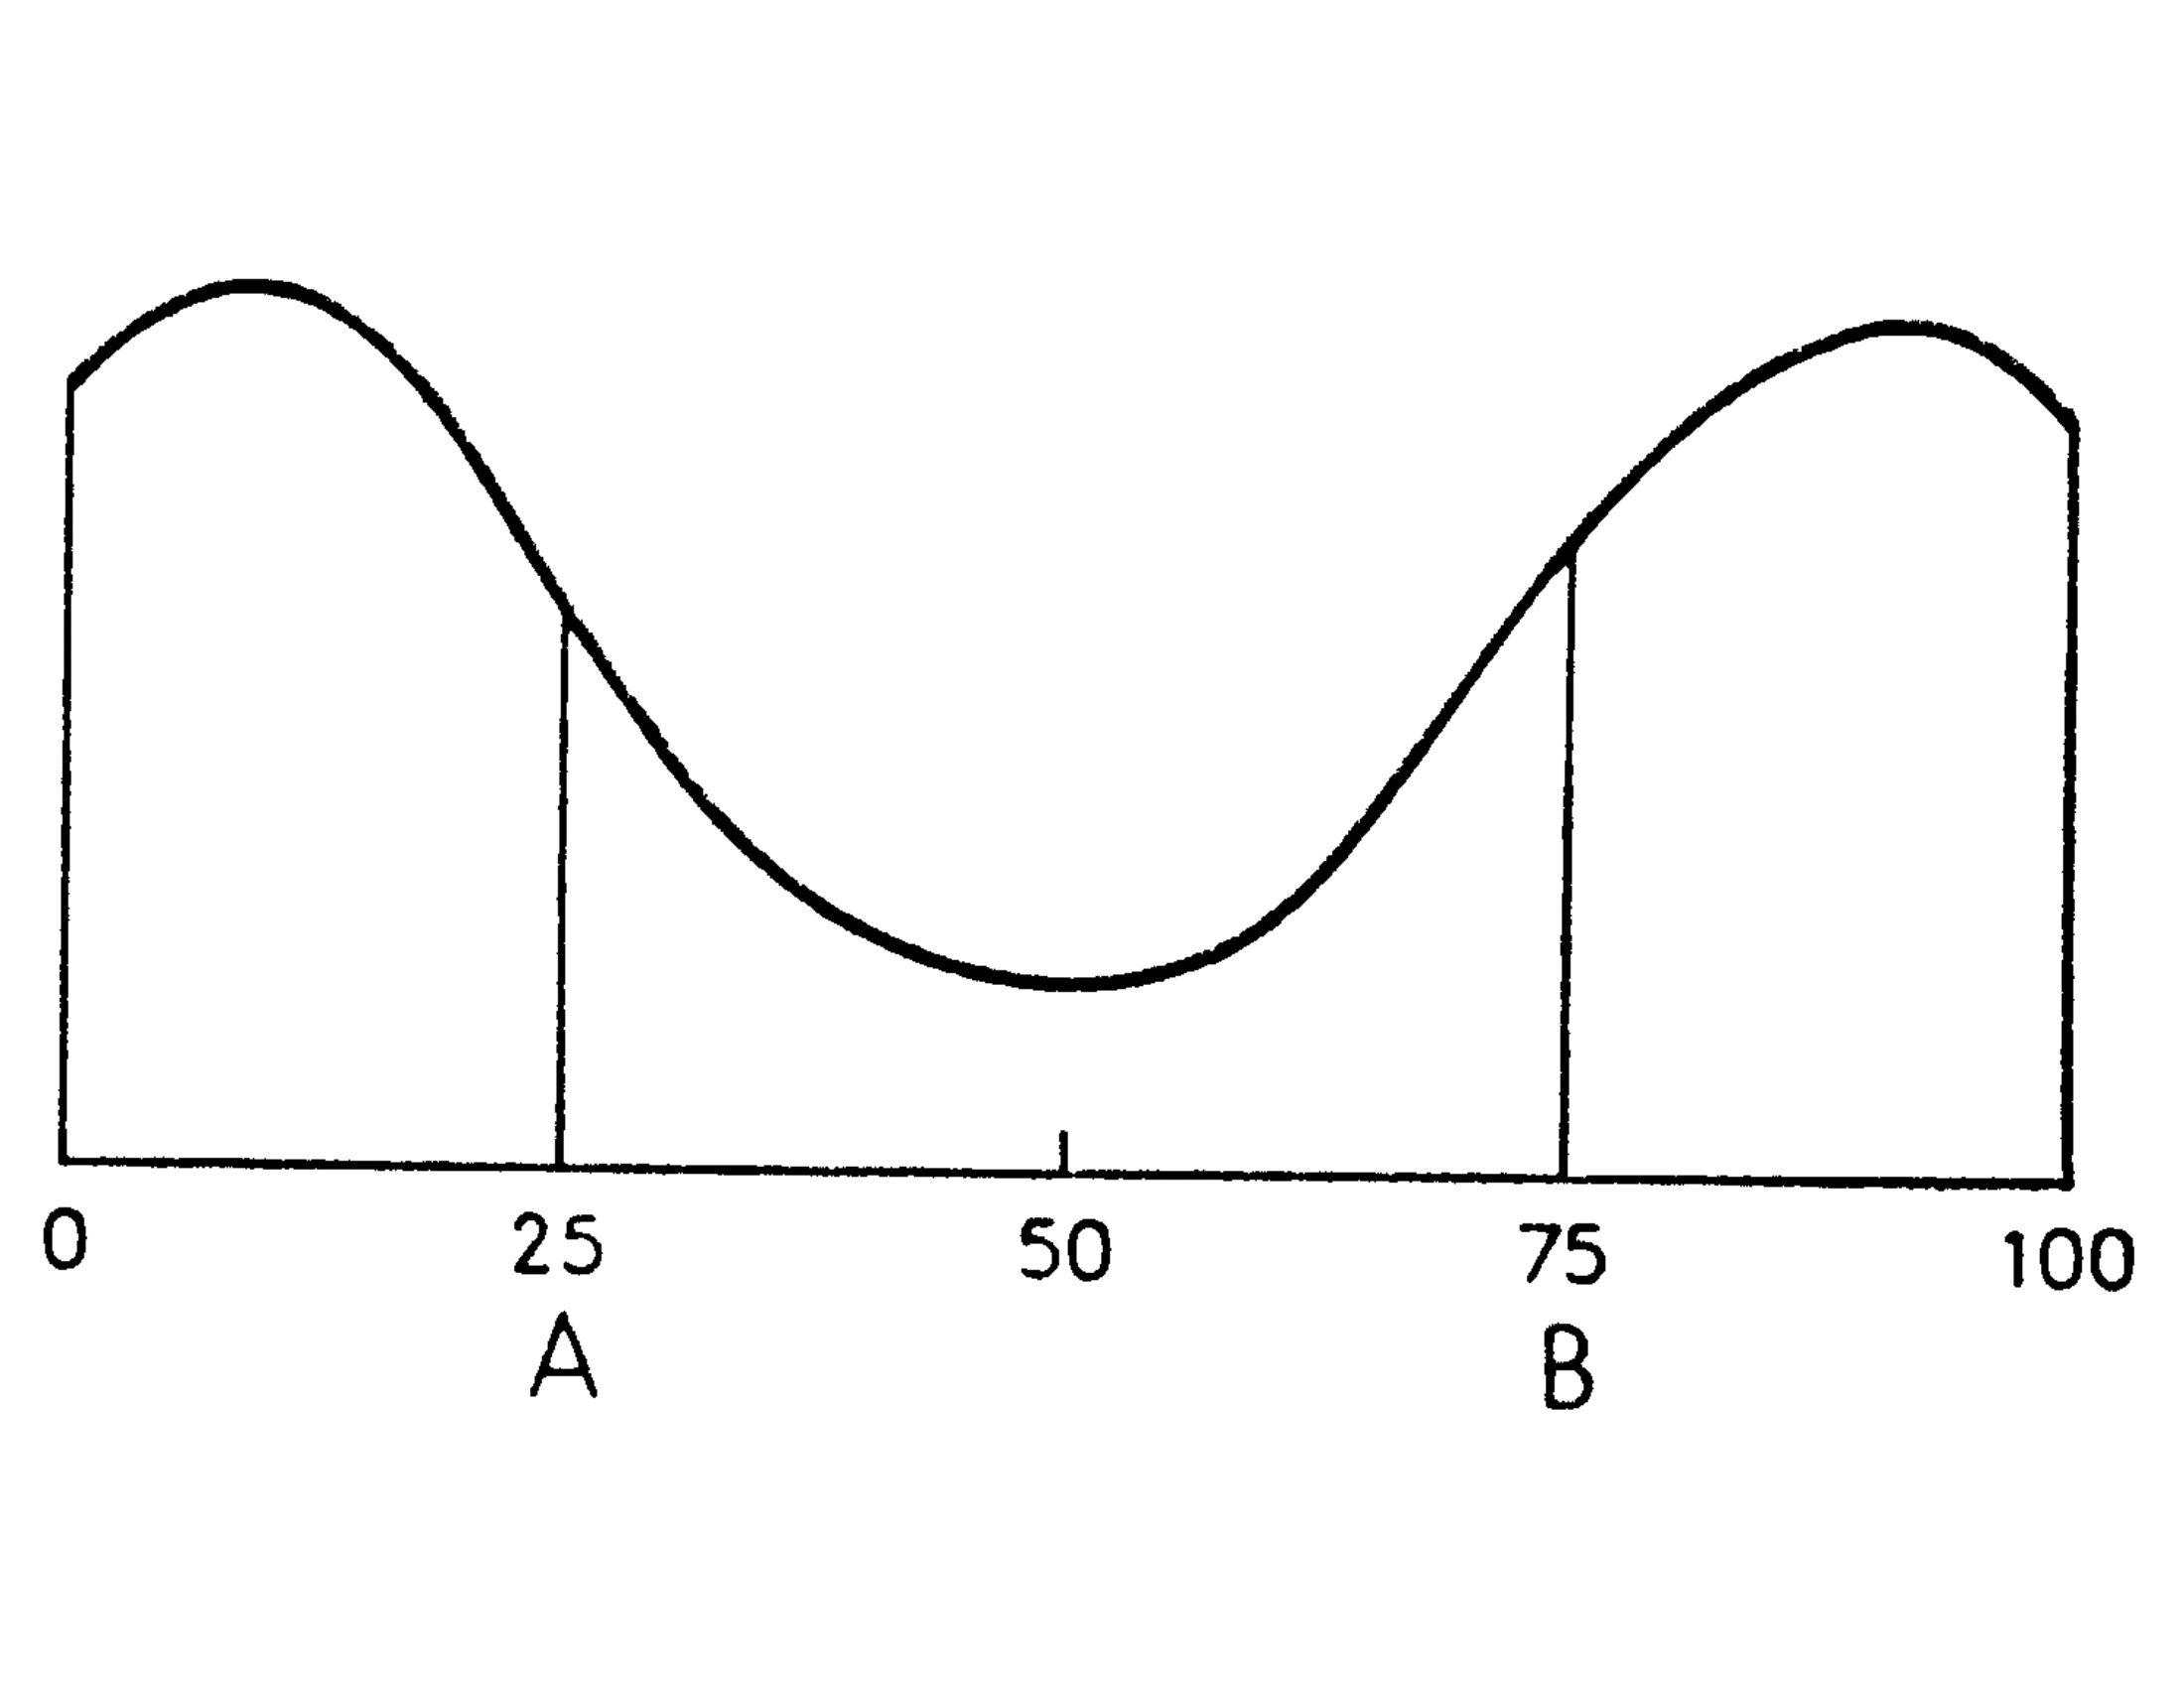
\includegraphics[scale=0.3]{downs6} \vspace{-1cm}
  \caption{Distribución de votantes - Electorado polarizado}
  \label{fig:3}
\end{figure}
\end{frame}

 \begin{frame}\frametitle{Competencia electoral: Downs (cont.)}
  \begin{figure}[htbp] \vspace{-1cm}
  \centering
  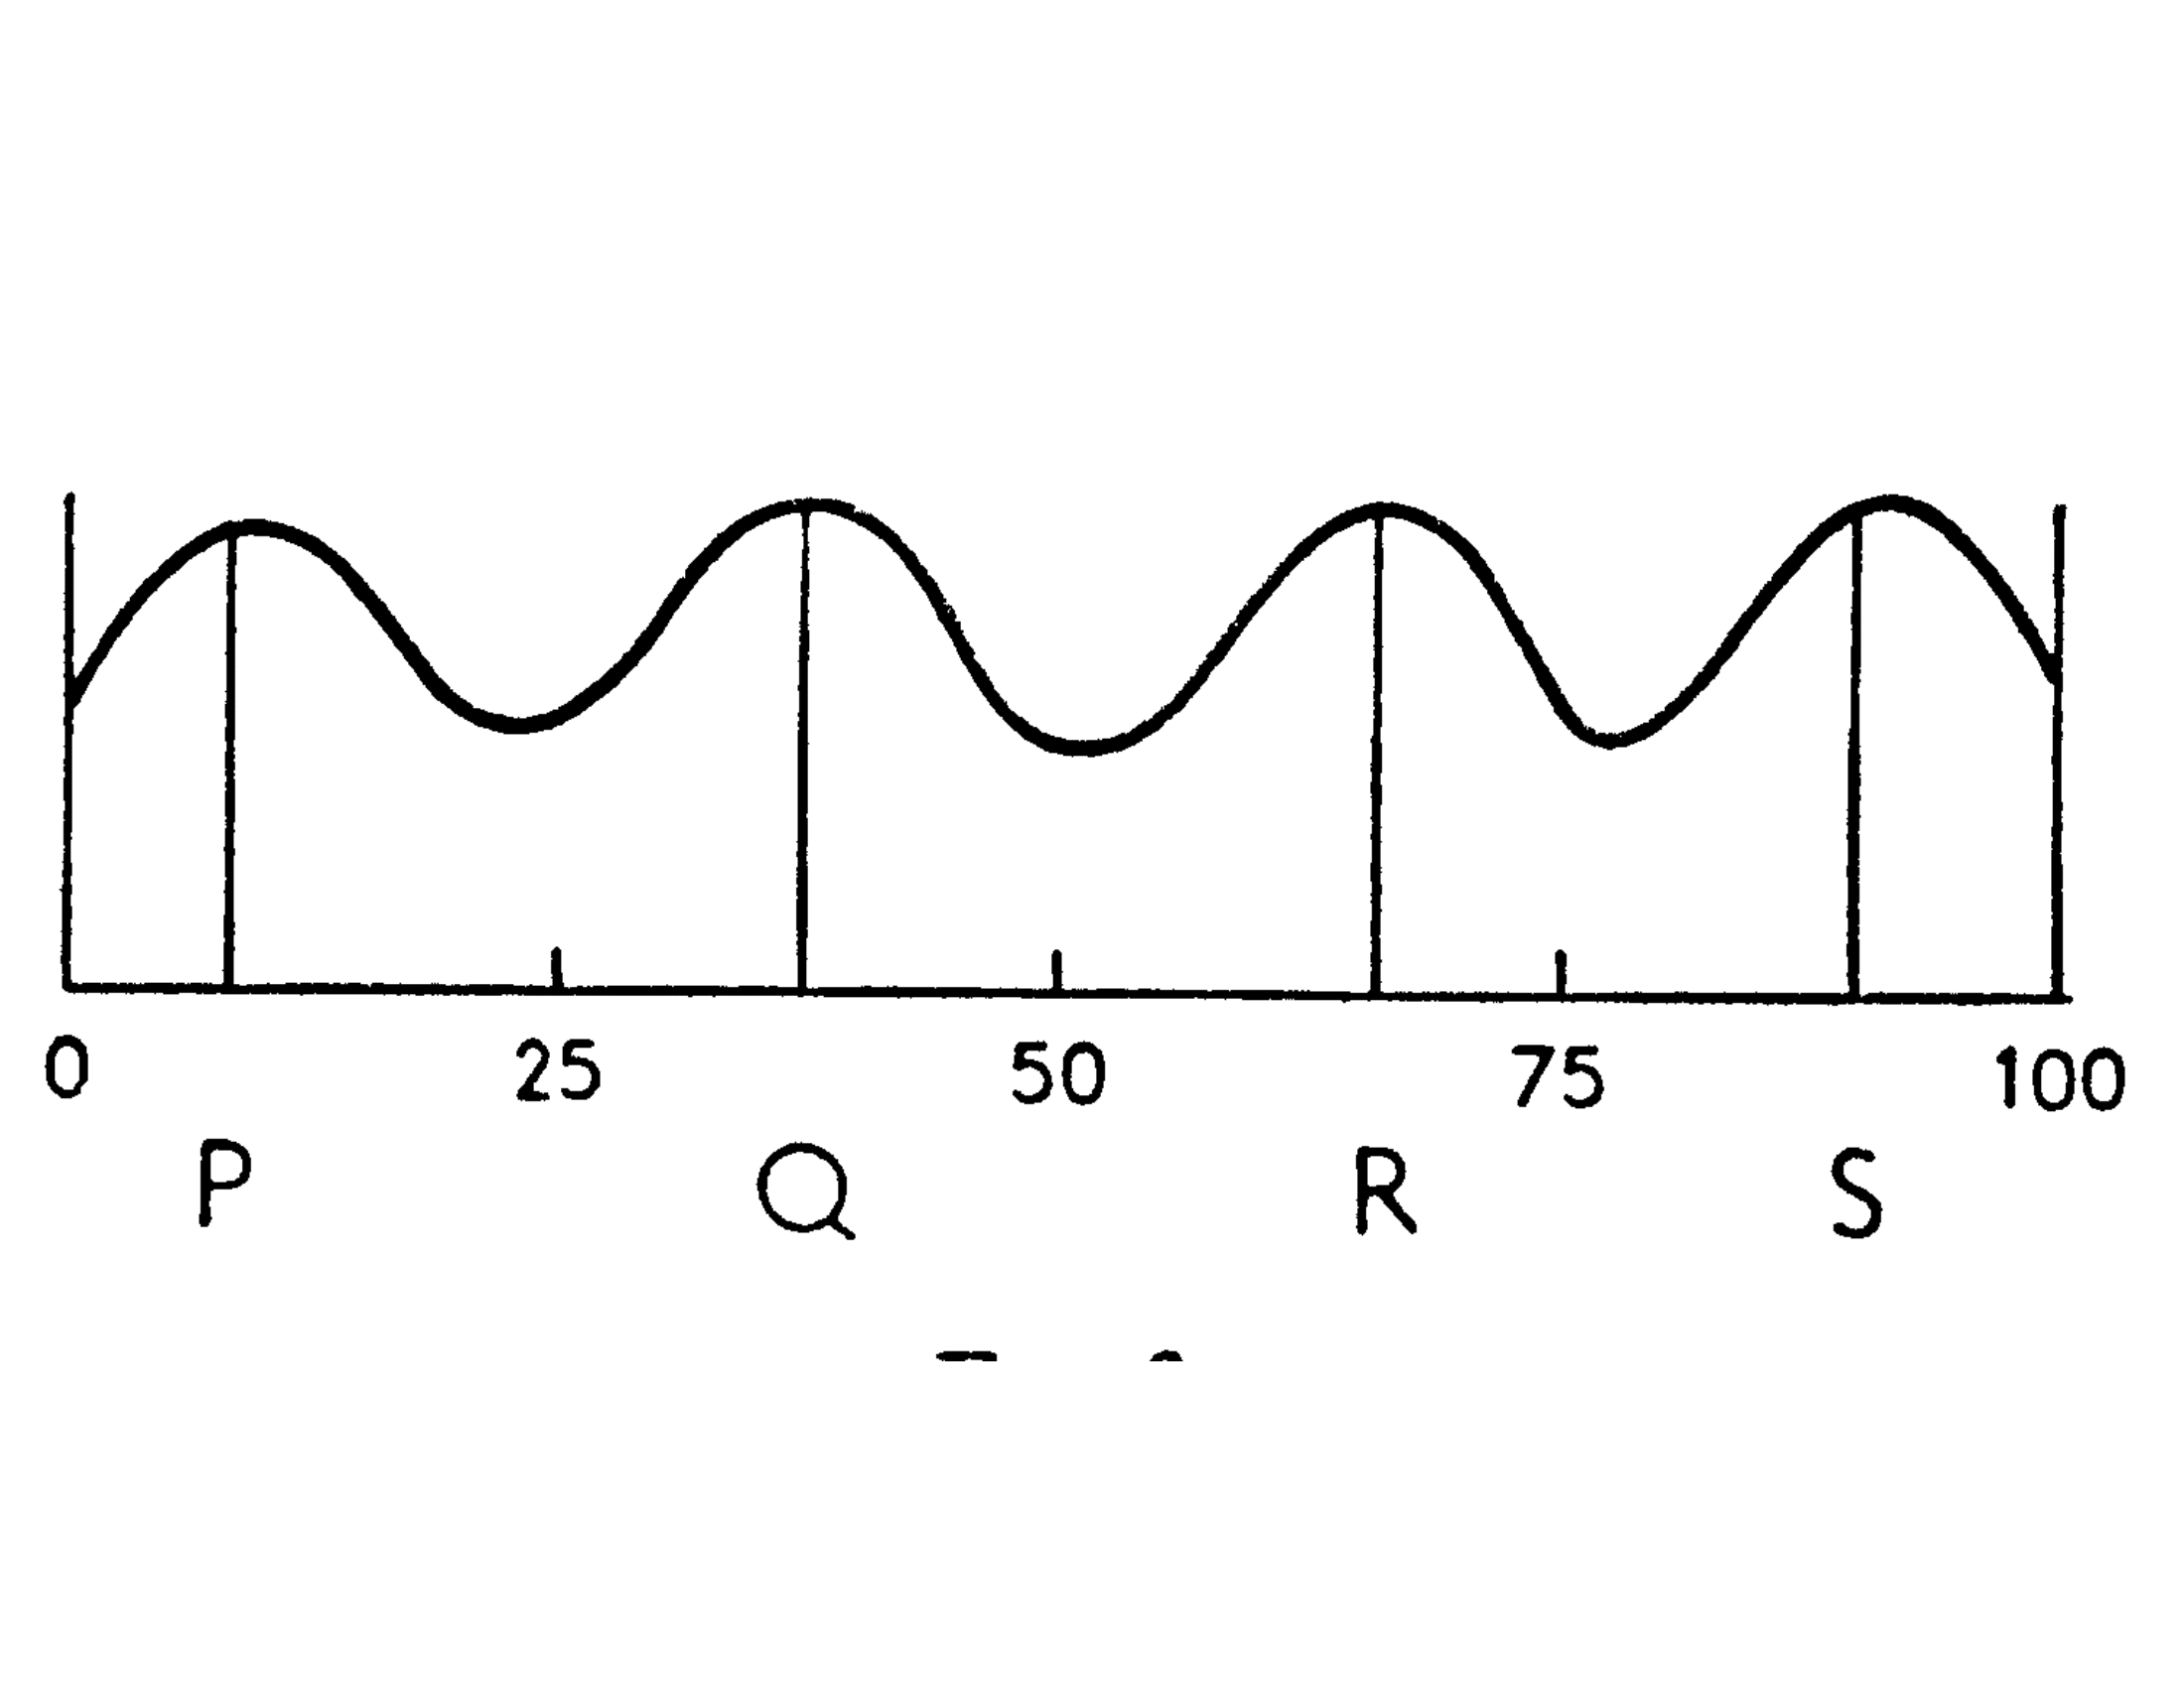
\includegraphics[scale=0.3]{downs7} \vspace{-1cm}
  \caption{Distribución de votantes - Electorado multimodal}
  \label{fig:3}
\end{figure}
    \end{frame}


\begin{frame}\frametitle{Competencia electoral: Downs (cont.)}
  \begin{itemize}
  \item Políticas estables en una democracia bi-partidista
    requiere distribucion normal
    $\longrightarrow$ los partidos tienden a parecerse. La \textit{identidad} del partido no importa.
    \item Si votantes polarizados, cambio en \textit{identidad} del
      ganador implica cambio en la política. Si continuidad
      $\longrightarrow$ oposición busca desestabilizar; si alternancia $\longrightarrow$ inestabilidad
      \item Si distribución multimodal $\longrightarrow$ sistema
        multi-partido. Cada partido se posiciona en una ``moda''. Implica mayor rango de opciones, mayor rol
        de ideología y menor coherencia $\longrightarrow$ gobierno de coaliciones
    \end{itemize}
  \end{frame}

    
    
\begin{frame}\frametitle{Aplicación I: Competencia electoral}
\begin{itemize}
\item Existe 3 (tres) grupos políticos, \textbf{liberal}, \textbf{de
    centro} y \textbf{socialdemocrata} que deben decidir sobre el
  nivel de gast [alto (A), medio (M) y bajo (B)] del sector público con las siguientes preferencias:
\end{itemize}
\begin{figure}[htbp] \vspace{-1cm}
  \centering
  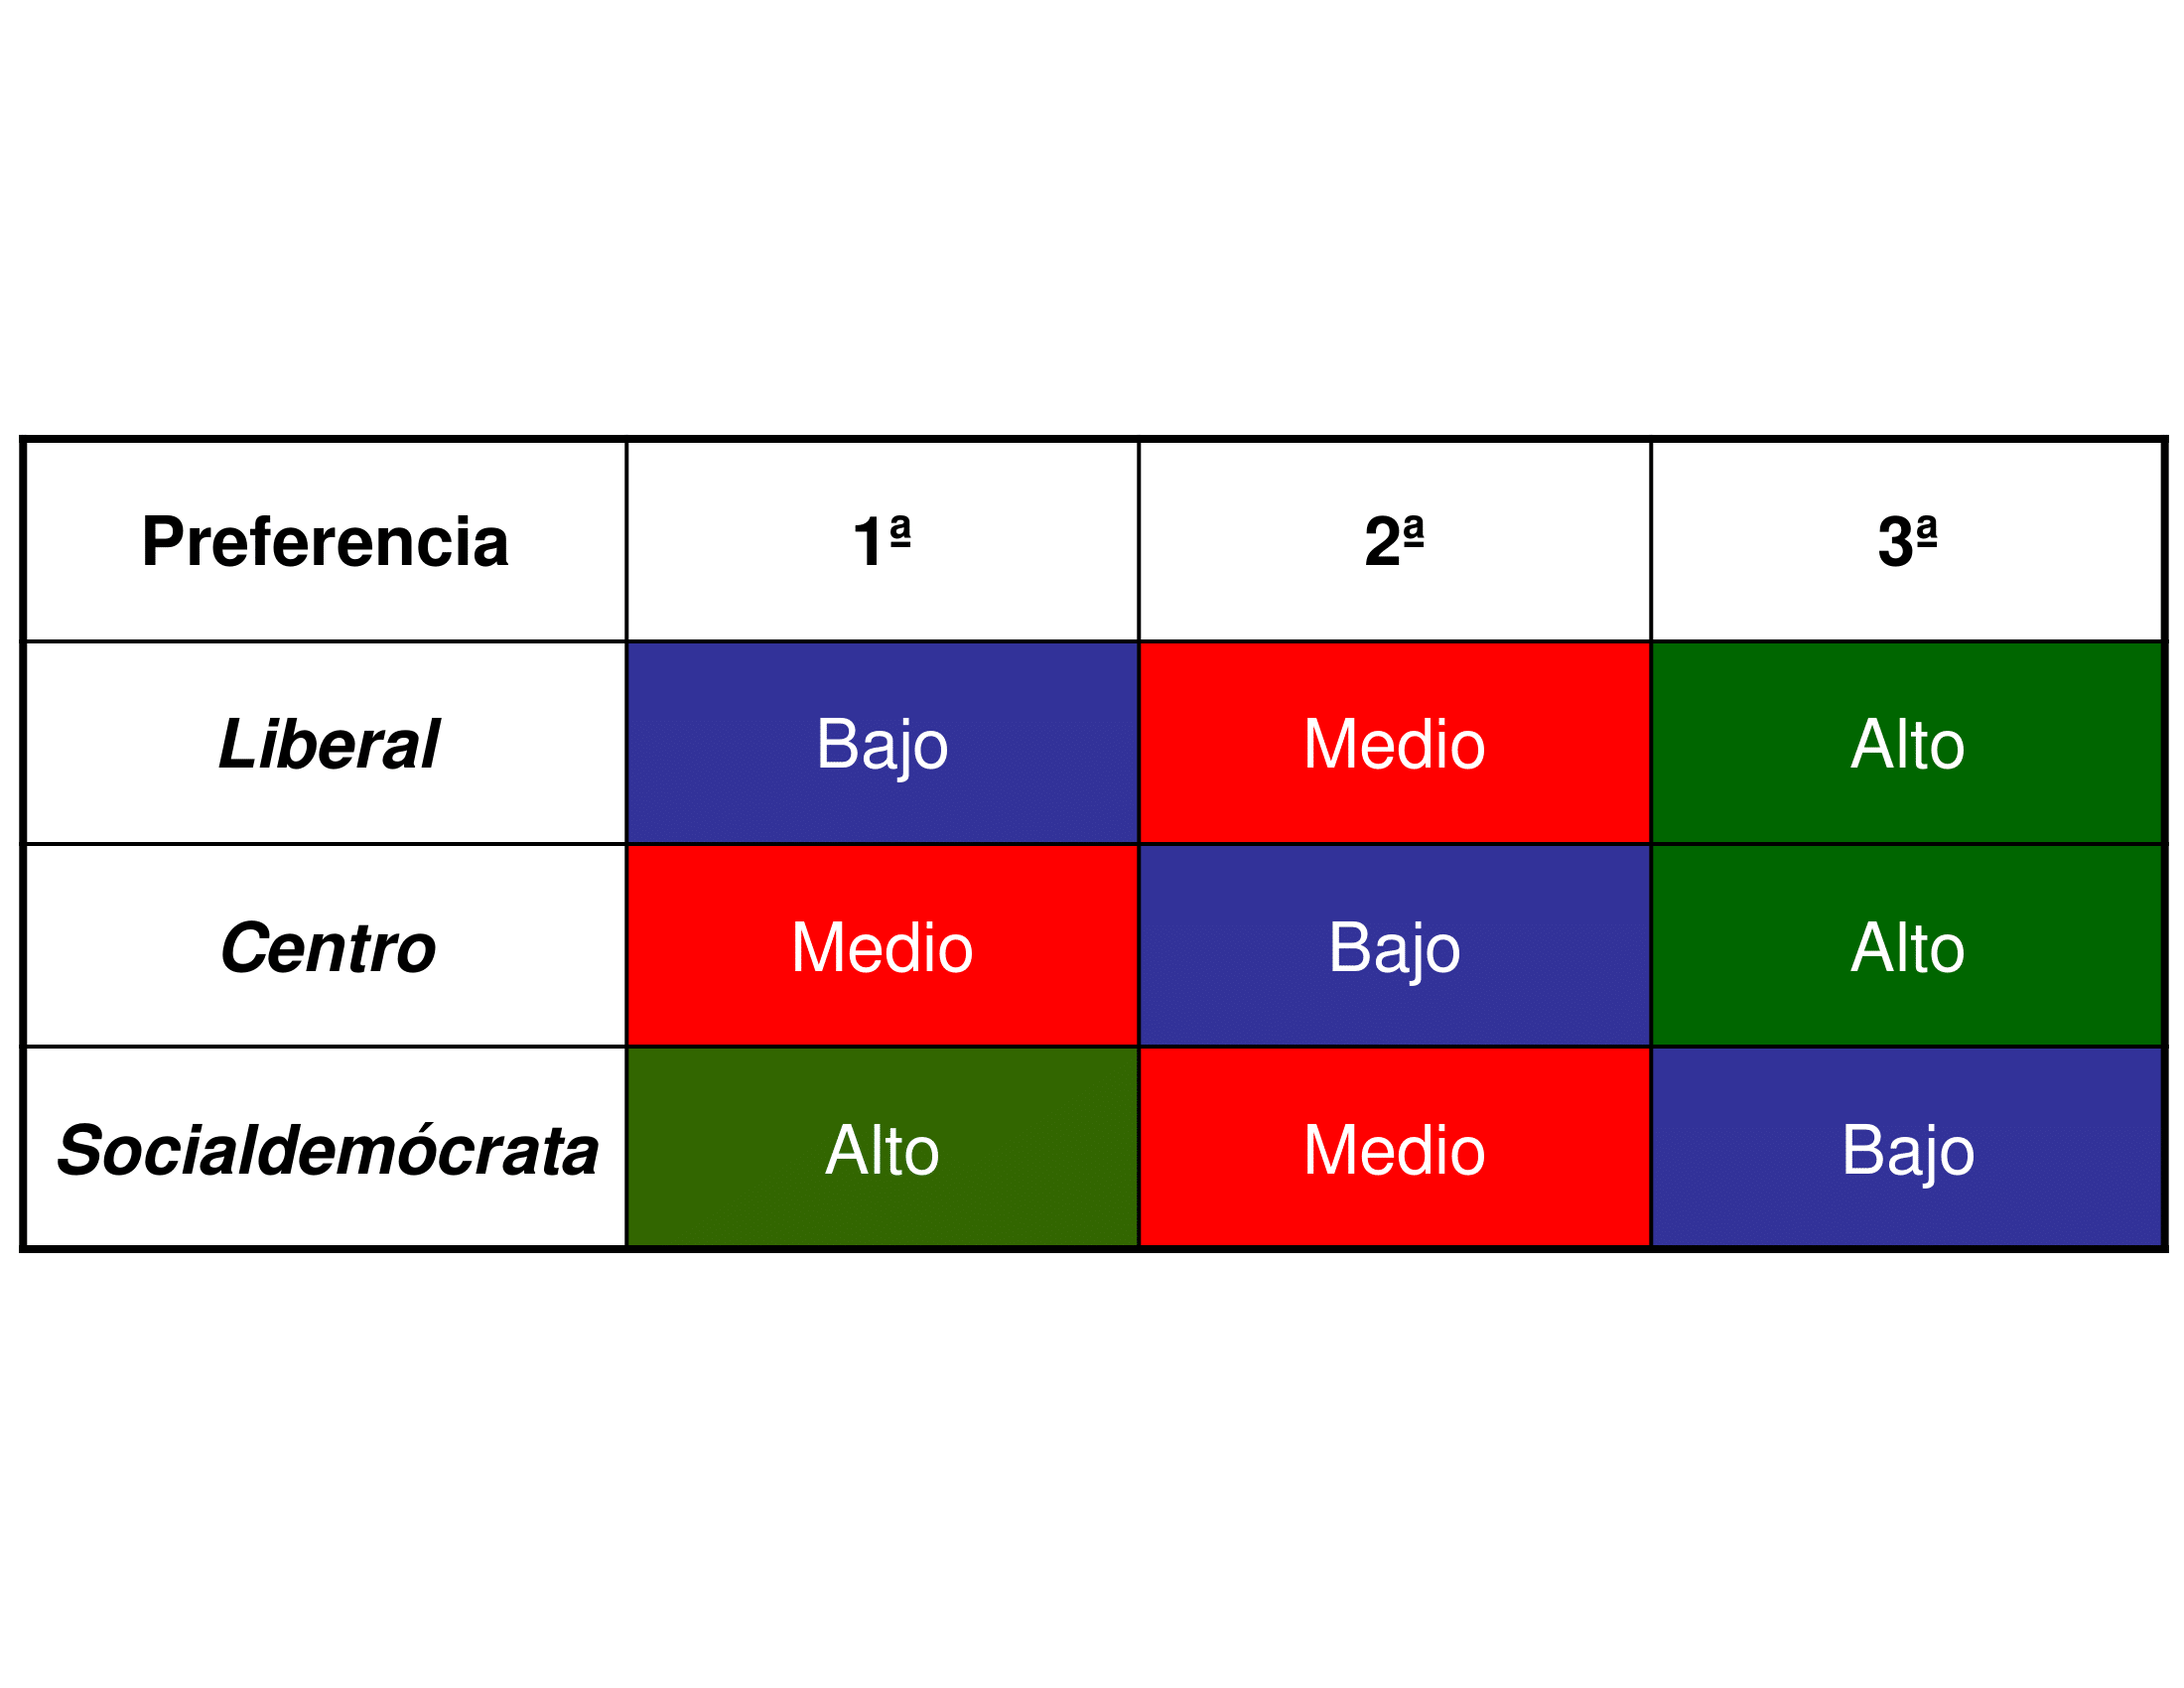
\includegraphics[scale=0.25]{ideologia} \vspace{-1cm}
  \caption{Ideología y preferencias de tres grupos de votantes}
  \label{fig:3}
\end{figure}
\end{frame}


\begin{frame}\frametitle{Aplicación I: Competencia electoral (cont.)}
\begin{itemize}
\item Sea cual fuere el orden en que se presenten las alternativas, se
  aprobará un nivel medio de gasto $\longrightarrow$ es la opción
  preferida por el votante mediano
\item Verifique por que:
\begin{itemize}\itemsep 5pt
\item A vs M $\Rightarrow$ M; M vs B $\Rightarrow$ M
\item A vs B $\Rightarrow$ B; B vs M $\Rightarrow$ M
\item M vs B $\Rightarrow$ M; M vs A $\Rightarrow$ M
\end{itemize}
\item El modelo no funciona cuando:
\begin{itemize}\itemsep 5pt
\item hay más de
  una dimensión (decentralización y desregulación; derechos civiles y
  derechos sociales)
\item las preferencias no son de pico único (unimodales)
\end{itemize}
\end{itemize}
\end{frame}


\begin{frame}\frametitle{Aplicacion II: Pre-electoral USA}
\begin{itemize}
\item Dos partidos políticos: Demócratas y Republicanos
\item Acciones posibles: cada partido puede colocarse en
  \textit{cualquier} posición del arco político
\item Electores: hay 200 millones de electores. 
\item Cada persona tiene preferencias de modo que vota a aquél partido
  que esté más cerca de su punto ideal. 
\item Suponemos que los electores se distribuyen de forma uniforme por
  todo el arco ideológico (grafico 1). 
\end{itemize}
\end{frame}

\begin{frame}\frametitle{Aplicacion II: Pre-electoral USA (cont.)}
\begin{itemize}
\item Suponemos originalmente las posiciones D y R están:
\end{itemize}
\begin{figure}[htbp] \vspace{-1cm}
  \centering
  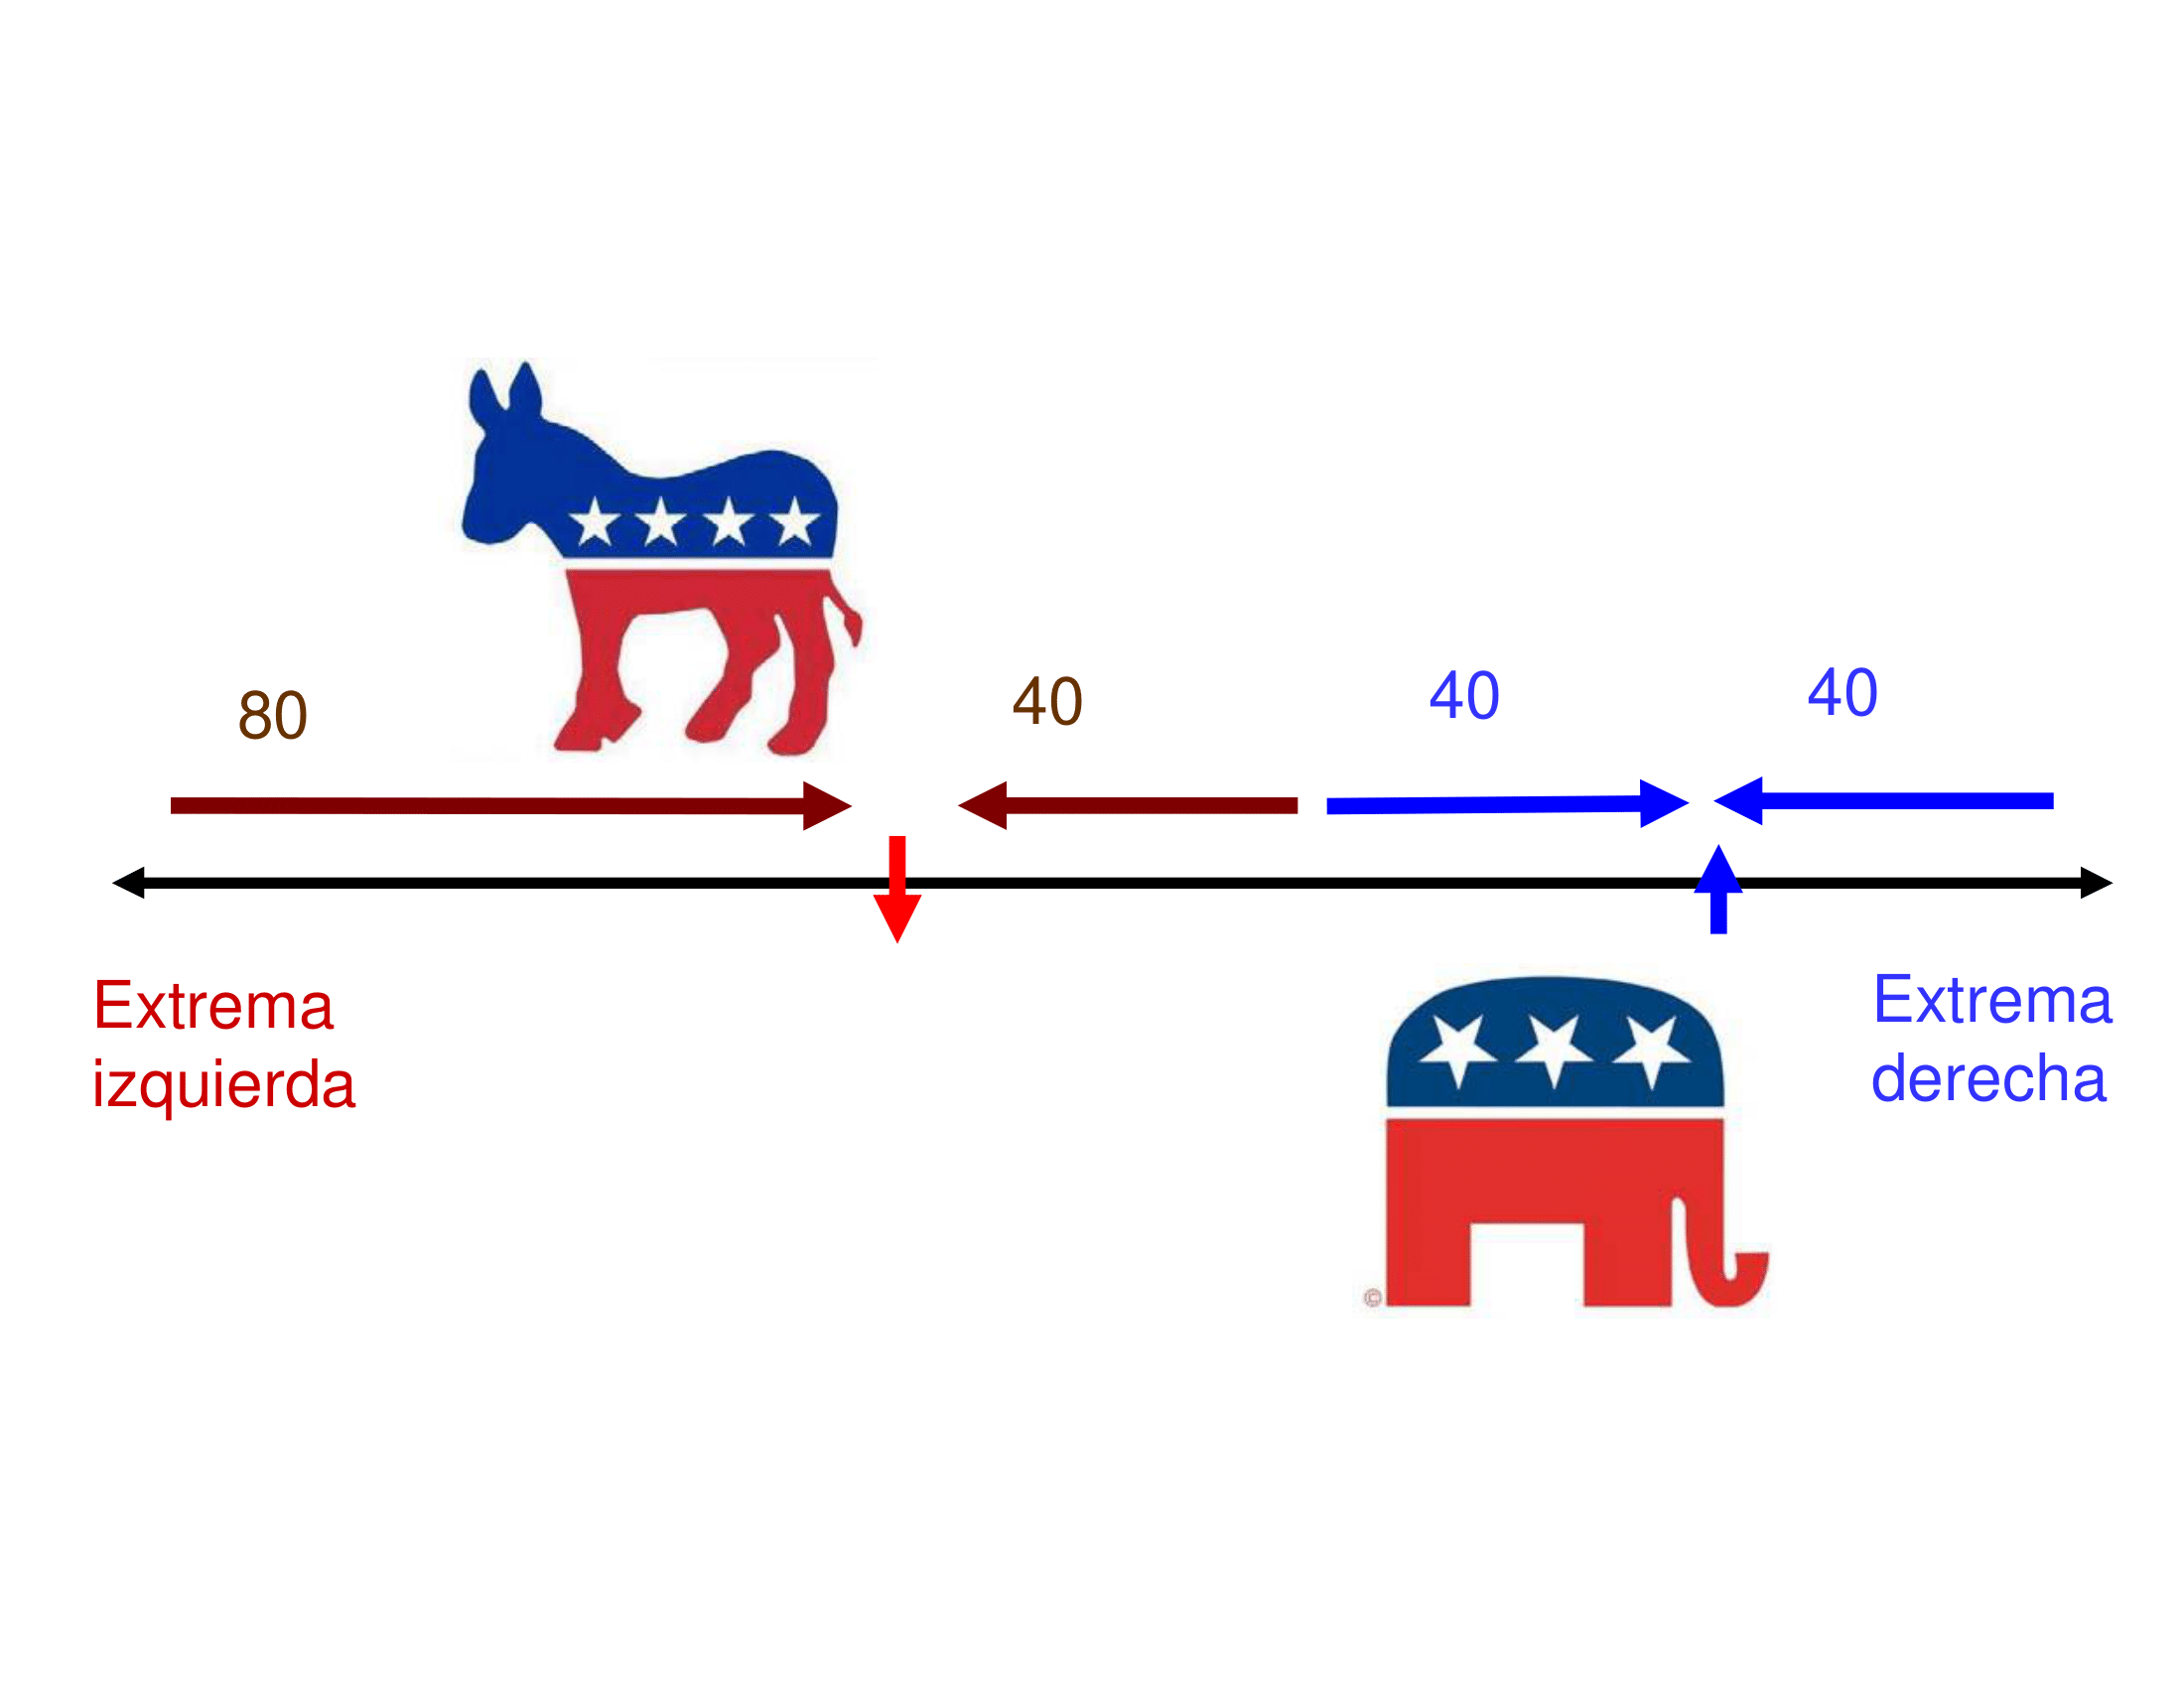
\includegraphics[scale=0.3]{downs1} \vspace{-1cm}
  \caption{Secuencia posicionamiento partidos}
  \label{fig:3}
\end{figure}
\end{frame}


\begin{frame}\frametitle{Aplicacion II: Pre-electoral USA (cont.)}
\begin{itemize}
\item Los Republicanos tienen incentivo a moverse hacia la izquierda
 \end{itemize}
\begin{figure}[htbp] \vspace{-1cm}
  \centering
  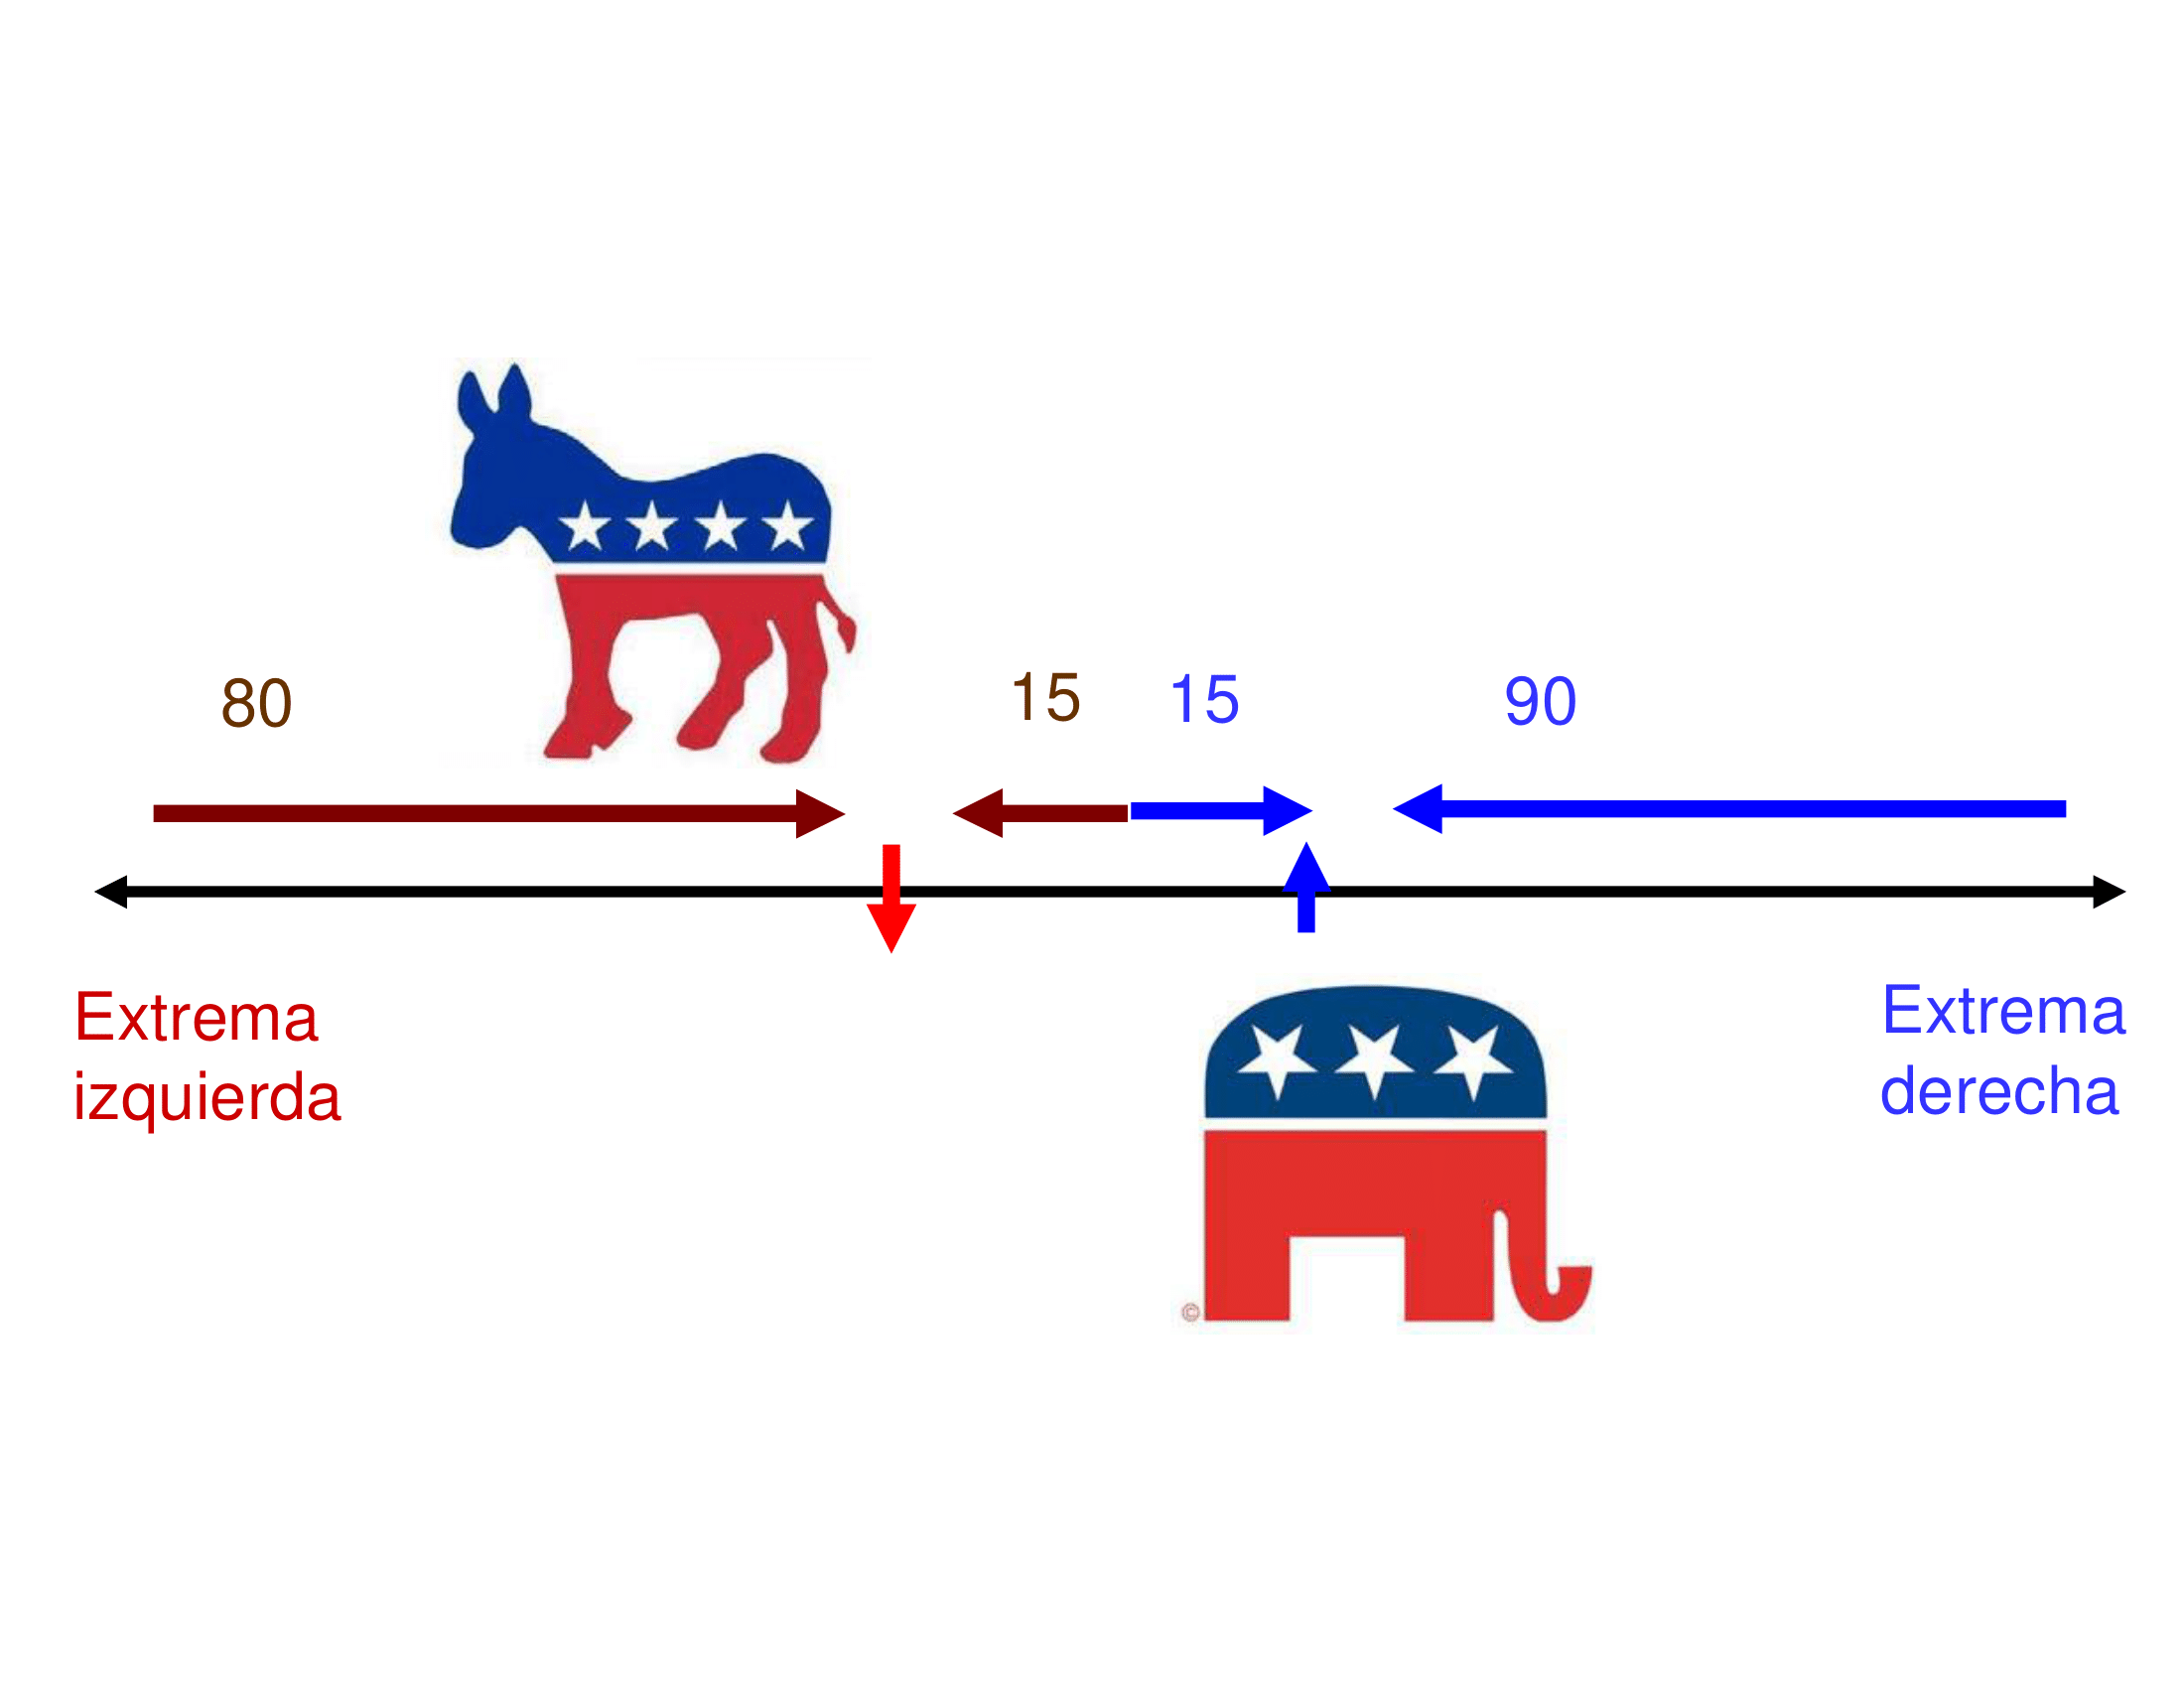
\includegraphics[scale=0.3]{downs2} \vspace{-1cm}
  \caption{Secuencia posicionamiento partidos}
  \label{fig:3}
\end{figure}
\end{frame}


\begin{frame}\frametitle{Aplicacion II: Pre-electoral USA (cont.)}
\begin{itemize}
\item Y ahora los Democratas deciden colocarse en el medio!
 \end{itemize}
\begin{figure}[htbp] \vspace{-1cm}
  \centering
  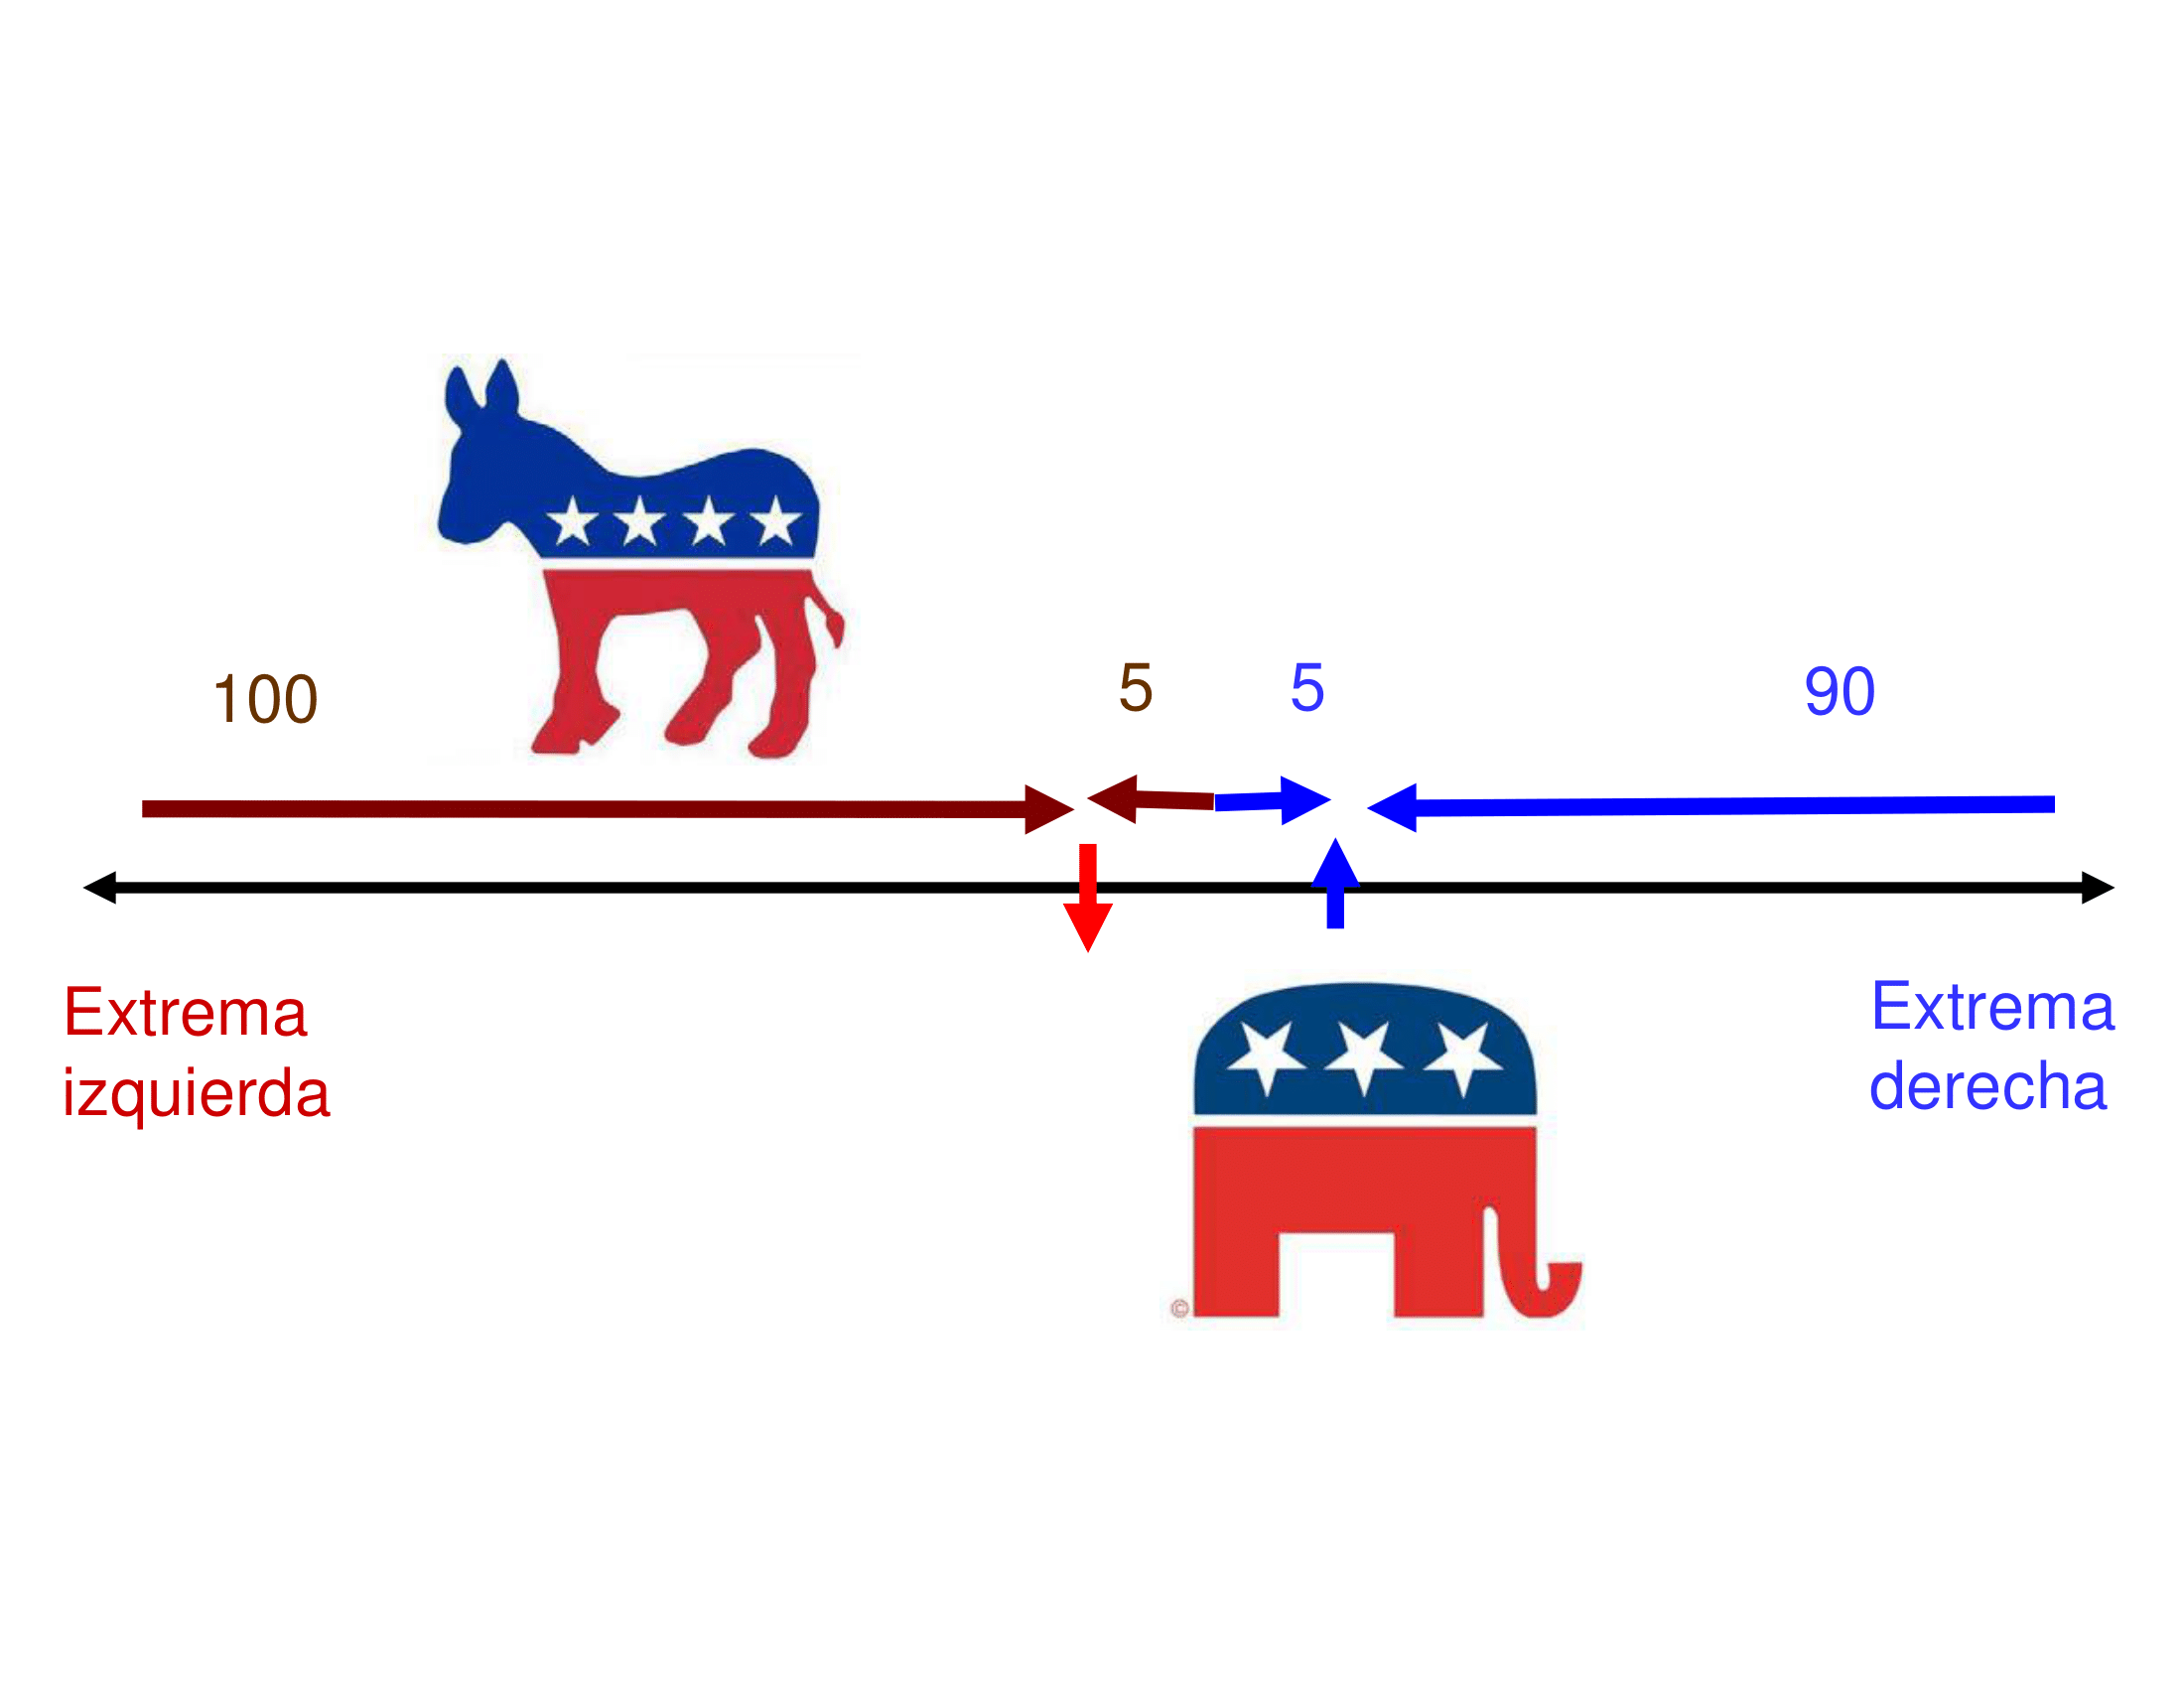
\includegraphics[scale=0.3]{downs3} \vspace{-1cm}
  \caption{Secuencia posicionamiento partidos}
  \label{fig:3}
\end{figure}
\end{frame}


\begin{frame}\frametitle{Aplicacion II: Pre-electoral USA (cont.)}
\begin{itemize}
\item Pero los Republicanos están perdiendo votos no estando en el
  medio, por lo que...también van al medio! 
 \end{itemize}
\begin{figure}[htbp] \vspace{-1cm}
  \centering
  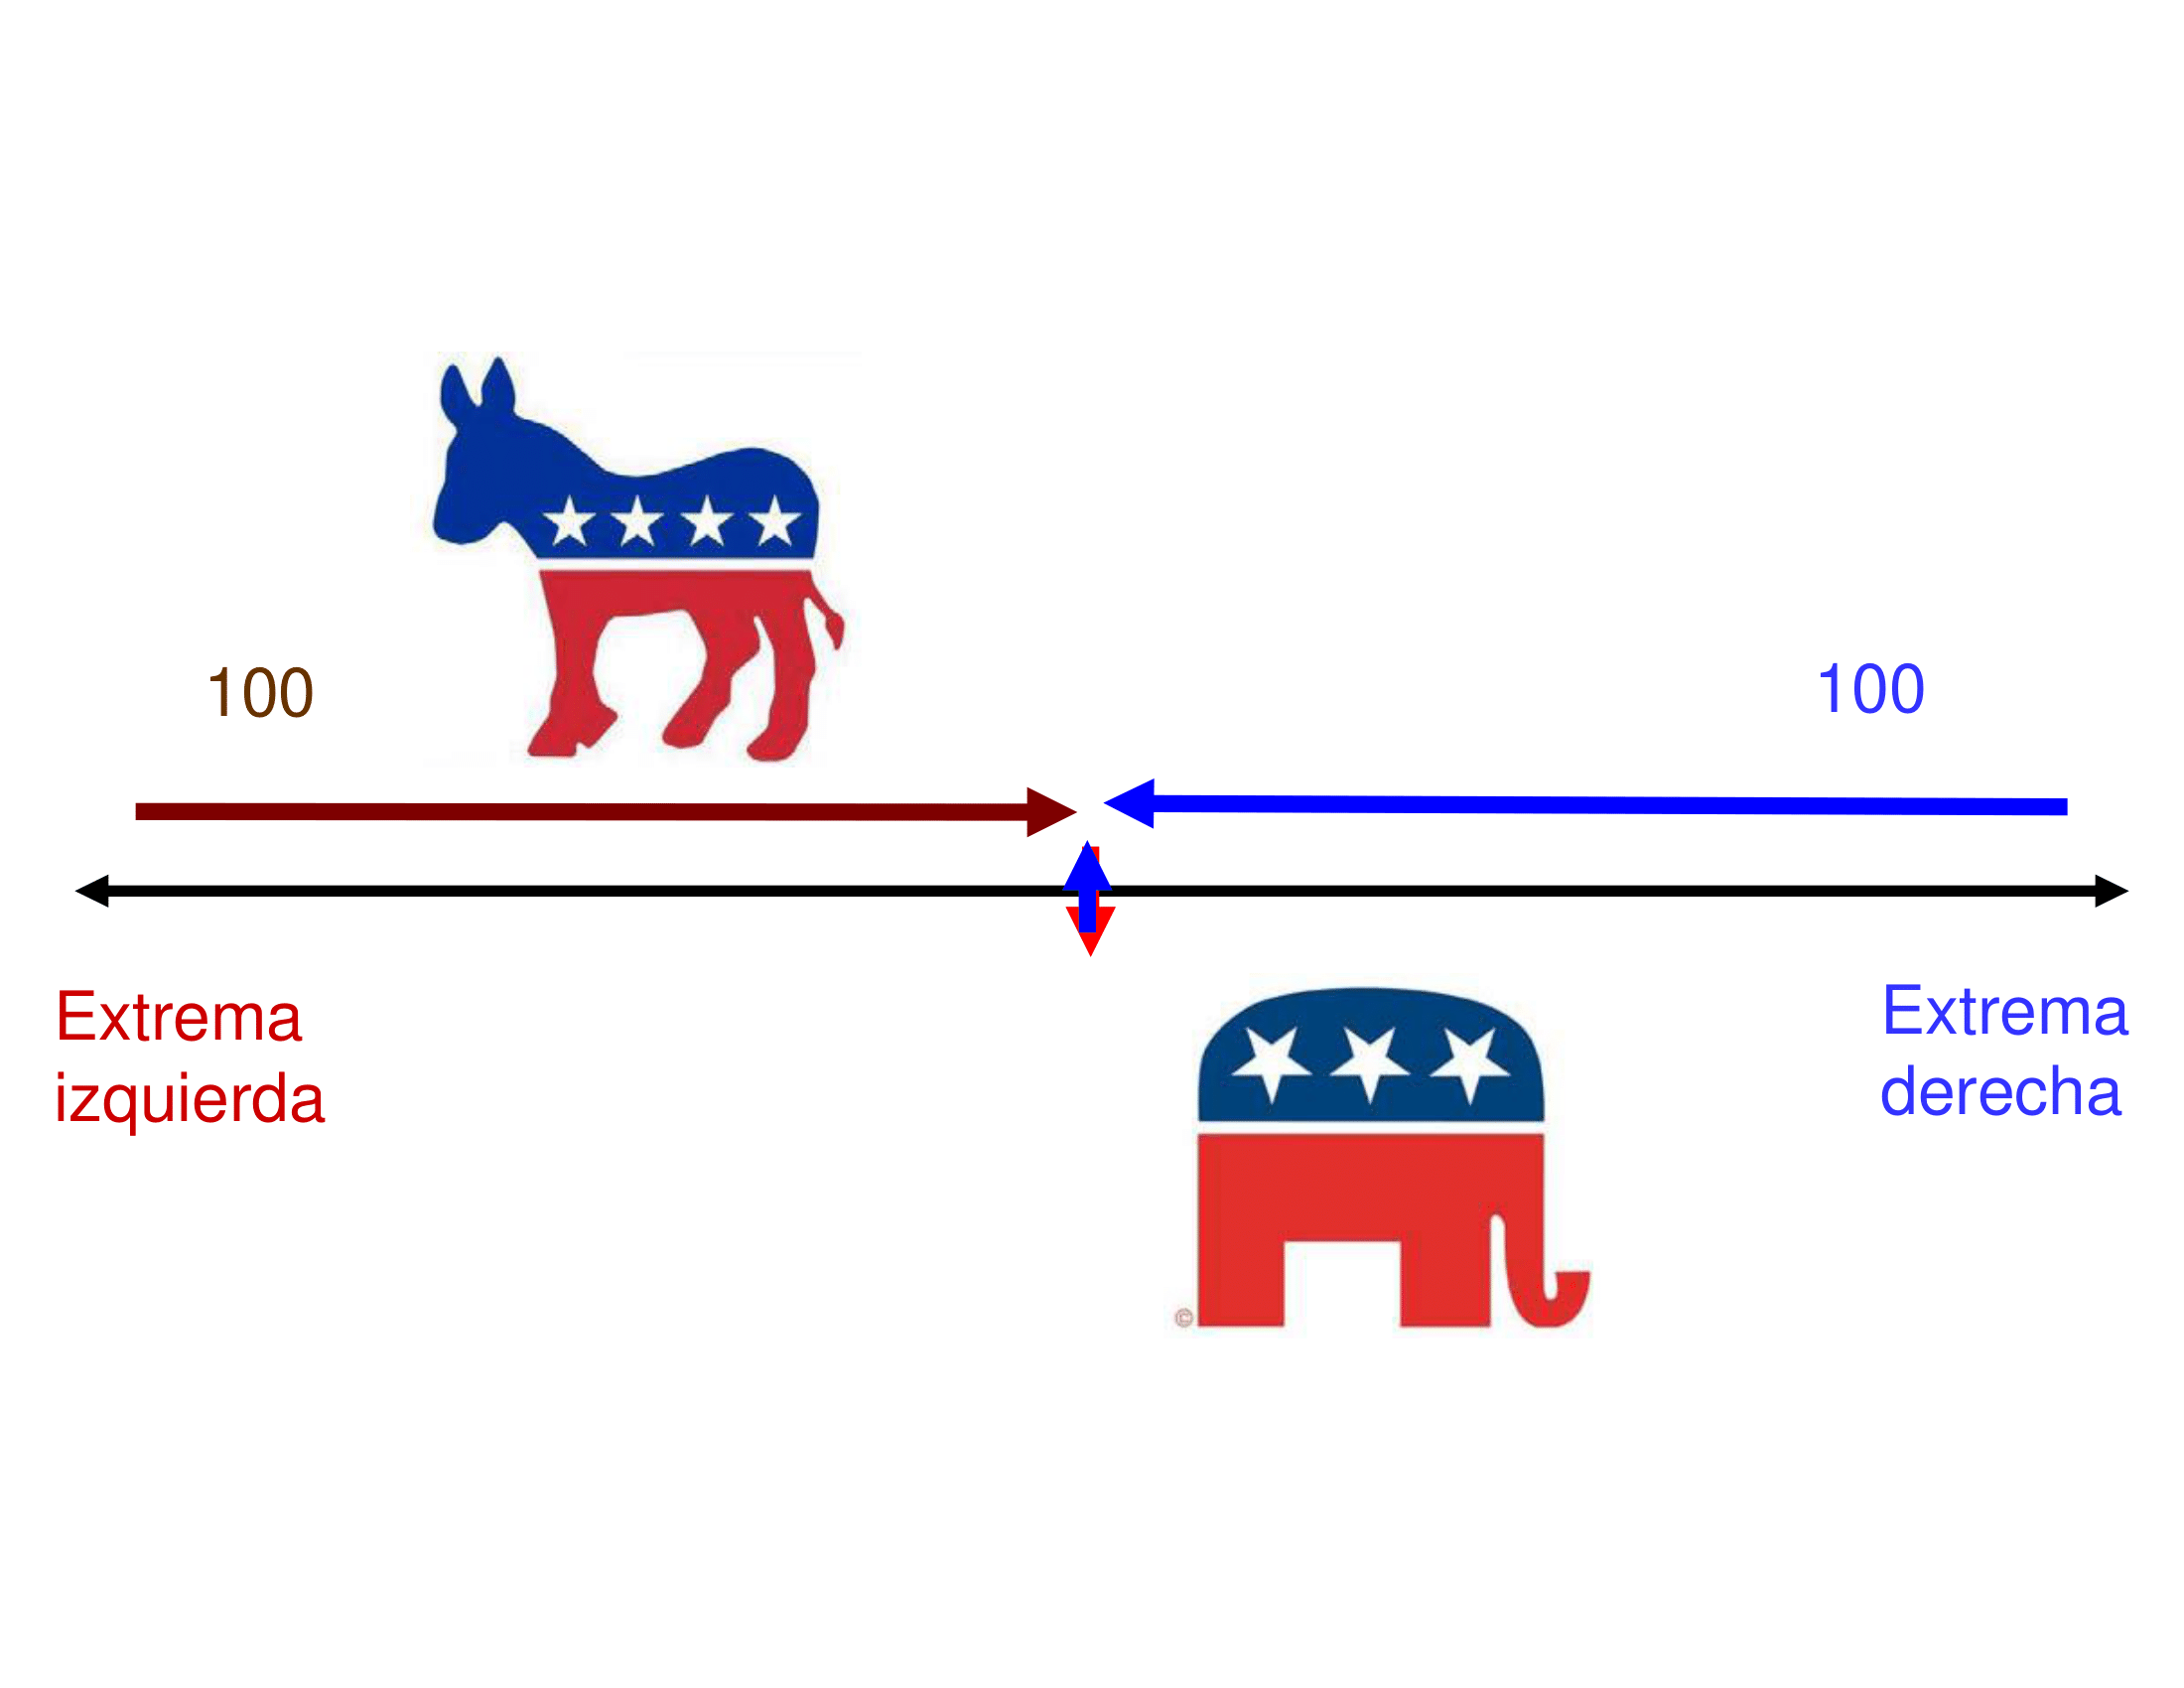
\includegraphics[scale=0.3]{downs4} \vspace{-1cm}
  \caption{Secuencia posicionamiento partidos}
  \label{fig:3}
\end{figure}
\end{frame}


\begin{frame}\frametitle{Aplicación III: ¿Qué alícuota fijar?}
\begin{itemize}
\item Suponga un gobierno que debe decidir el nivel de gasto e
  imposición. Existe un sólo impuesto $\longrightarrow$ el impuesto a
  la renta. Debe determinarse la alicuota, $\tau$. Si el ingreso
  individual es $y$, el ingreso después de impuestos es $y(1-\tau)$.
\item La imposición tiene un costo. Supongamos que el costo
  (distorsión) del impuesto es igual a $\delta \tau^2$. 
\item El votante mediano quiere maximizar su consumo (depende del
  ingreso después de impuestos, del gasto público y del costo de la
  imposición).
\end{itemize}
\end{frame}


\begin{frame}\frametitle{Aplicación III: ¿Qué alícuota fijar? (cont.)}
\begin{itemize}\itemsep 15pt
\item El consumo final de un persona viene dado por:
\begin{equation}
C=y(1-\tau)+\tau y_{avg}-\delta \tau^2
\end{equation}
\item y la alícuota óptima viene dada por:
\begin{equation}
\tau=\frac{y_{avg}-y_{median}}{2\delta}
\end{equation}
\item Note que la \textit{alícuota (y el tamaño del gobierno) son crecientes
  en la \underline{diferencia} entre el ingreso promedio y el ingreso mediano}. 
\item Clave $\longrightarrow$ políticos toman decisiones
  basadas en votante mediano; tasas
  medias están basadas en el ingreso medio. 
\end{itemize}
\end{frame}

\begin{frame}\frametitle{Aplicacion III: ¿Qué alícuota fijar? (cont.)}
\begin{itemize}
\item Suponga 5 personas (y suponga $\delta=0.5$). Sea $y={0,1,2,3,4}$
\begin{itemize}\itemsep 0pt \medskip
\item Mediana? 2 ---  Media? 2 --- $\tau$? 0
\item $C=y(1-\tau)+\tau y_{avg}-\delta \tau^2$ $\Rightarrow$ $C=2(1-0)+0-0=2$
\end{itemize}
\item Ahora, con $y={0,1,2,3,9}$
\begin{itemize}\itemsep 0pt \medskip
\item Mediana? 2 --- Media? 3 --- $\tau$? 1
\item $C=y(1-\tau)+\tau y_{avg}-\delta \tau^2$ $\Rightarrow$ $C=2(1-1)+1*3-0.5=2.5$
\end{itemize}
\item Ahora, con $y={0,1,2,3,59}$
\begin{itemize}\itemsep 0pt \medskip
\item Mediana? 2 --- Media? 13 --- $\tau$? 11
\item $C=y(1-\tau)+\tau y_{avg}-\delta \tau^2$ $\Rightarrow$ $C=2(1-11)+11*13-0.5*(11)^2=62.5$
\end{itemize}
\end{itemize}
\end{frame}


\begin{frame}\frametitle{Aplicacion III: ¿Qué alícuota fijar? (cont.)}
\begin{itemize}
\item ¿Qué esta ocurriendo? 
\begin{itemize}
\item Lo que sucede es que en este simple modelo \textit{la política está determinada por la
  diferencia entre el mediano y la media}
\item Esto implica que, por ejemplo, cuando existen grandes niveles de
  desigualdad (particularmente cuando hay personas extremadamente
  ricas como en el tercer caso), el votante mediano puede ganar mucho
  al fijar una alícuota mayor y poner impuestos sobre los ricos. 
\end{itemize}
\item ¿Por qué la alícuota era igual a cero en el caso 1 cuando el
  mediano y la media eran iguales?
\begin{itemize}\itemsep 5pt \medskip
\item El mediano no se beneficia en absoluto de que haya una alícuota
  (ver consumo). Como la imposición es costosa (distorsiva), la
  alícuota optima es igual a 0. 
\end{itemize}
\end{itemize}
\end{frame}


\begin{frame}\frametitle{Utilidad del teorema del votante mediano}
\begin{block}{Utilidad del teorema del votante mediano}
We appeal to this (median voter) theorem to capture the basic idea that
any government is likely to be responsive to the wishes of the majority when
key distributional issues are at stake. Even a dictator cannot completely
ignore social demands for fear of being overthrown. Thus, even in a
dictatorship, distributional issues affecting the majority of the population
will influence policy outcomes [Alesina and Rodrik (1994)]
\end{block}
\end{frame}


\section{Mas allá del votante mediano}


\begin{frame}\frametitle{}
\begin{block}{Políticos unidimensionales}
Thus politicians in our model never seek office as a means of carrying
out particular policies: their only goal is to reap the rewards of
holding office \textit{per se}. They treat policies purely as a means
to the attainment of their private ends, which they can reach only by
being elected [Anthony Downs, \textit{An economic theory of democracy}]
\end{block}
\begin{itemize}\itemsep 10pt
\item ¿Es esta una representación adecuada de los políticos en la vida
  real? Evidencia sugiere que no necesariamente. 
\item Los políticos también pueden interesarse por su
  posición de política preferida; influyen intereses especiales
\end{itemize}
\end{frame}


\begin{frame}\frametitle{Las leyes de Duverger}
\begin{block}{Ley 1}
Los sistemas de votación por mayoría en una elección conducen a un sistema bipartidista
\end{block}
\begin{block}{Ley 2}
Los sistemas de votación por representación proporcional conducen a un
sistema multipartidista. 
\end{block}
\begin{block}{Ley 3}
Los sistemas de votación por mayoría en 2 vueltas llevan a un
sistema multipartido con tendencia a formar coaliciones
\end{block}
\end{frame}


\begin{frame}\frametitle{Número efectivo de partidos}
  \begin{table}[htbp]
    \centering
    \begin{tabular}[htbp]{lccc}
      Country	&	no. of elections	&	ENP & Sistema	\\ \hline
Canada	&	21	&	3.07  & mayoría	\\ \hline
UK	&	17	&	2.37  & mayoría	\\ \hline
US	&	17	&	1.99  & mayoría	\\ \hline
Australia	&	27	& 2.60 &  2da vuelta	\\ \hline
France	&	14	&	4.31 & 2da vuelta	\\ \hline
Argentina & 4 & 4.47 & PR \\\hline
Brazil &  7 & 9.33 & PR  \\ \hline
    \end{tabular}
    \caption{Número efectivo de partidos}
    \label{tab:2}
  \end{table}
\end{frame}


\begin{frame}\frametitle{Polarización: políticas y plataformas}
\begin{itemize}
\item Si se cumple Downs, se esperaría un bajo grado de
  polarización en las plataformas políticas de la vida real. 
\item Datos del ``comparative manifesto dataset'' (2015), polarización
  medida en escala I-D. 
\end{itemize}
\begin{table}[htbp]
  \centering
  \begin{tabular}[htbp]{lcc}
    Country	&	no. Elections	&	polarization	\\ \hline
Canada	&	21	&	0.10	\\ \hline
UK	&	17	&	0.15	\\ \hline
US	&	17	&	0.08	\\ \hline
Australia	&	27	&	0.16	\\ \hline
France	&	14	&	0.21	\\ \hline
  \end{tabular}
  %\caption{Grado de polarización en las políticas}
  \label{tab:3}
\end{table}
\end{frame}



\begin{frame}\frametitle{Evidencia I: Nominate Scores}
  \begin{figure}[htbp]
    \centering
    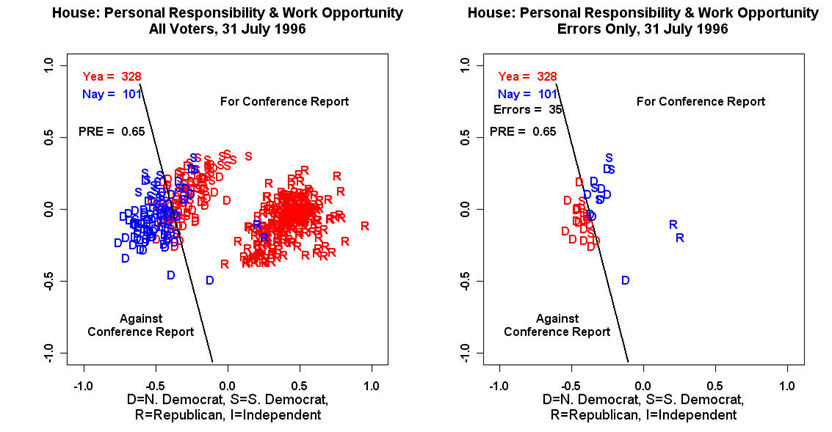
\includegraphics[scale=0.38]{nominate1}
    \caption{Posiciones legisladores EEUU}
    \label{fig:nominate1}
  \end{figure}
\end{frame}


\begin{frame}\frametitle{Evidencia I: Nominate Scores (cont.)}
  \begin{figure}[htbp]
    \centering
    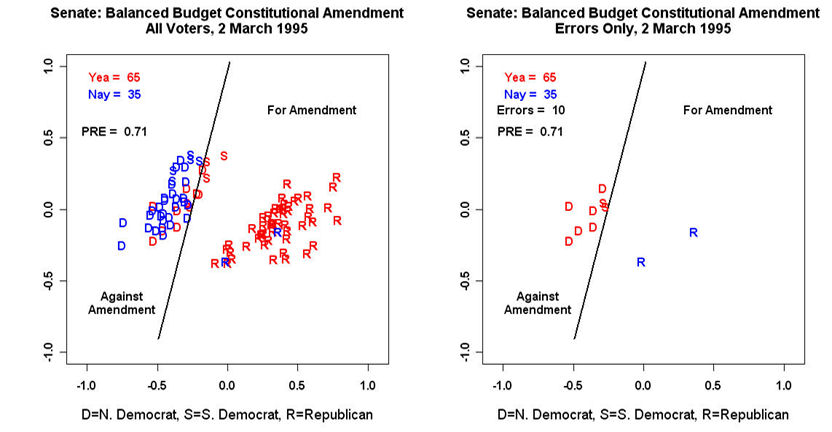
\includegraphics[scale=0.38]{nominate2}
    \caption{Posiciones legisladores EEUU}
    \label{fig:nominate2}
  \end{figure}
\end{frame}


\begin{frame}\frametitle{Evidencia I: Nominate Scores (cont.)}
  \begin{figure}[htbp]
    \centering
    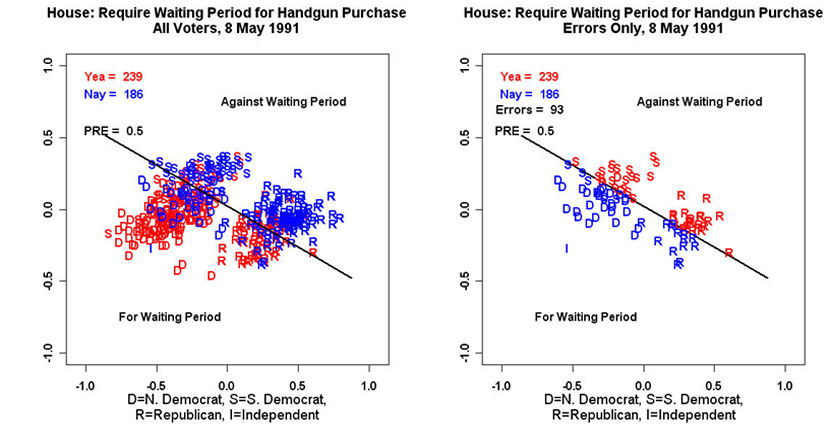
\includegraphics[scale=0.38]{nominate3}
    \caption{Posiciones legisladores EEUU}
    \label{fig:nominate3}
  \end{figure}
\end{frame}

\begin{frame}\frametitle{Evidencia II: Congreso Argentino}
\begin{figure}[htbp]
    \centering
    \includegraphics[scale=0.38]{dv1}\vspace{-0.75cm}
    \caption{Votaciones diputados argentinos}
    \label{fig:dv1}
  \end{figure}
\end{frame}


\begin{frame}\frametitle{Evidencia II: Congreso Argentino (cont.)}
\begin{figure}[htbp]
    \centering
    \includegraphics[scale=0.38]{dv2}\vspace{-0.75cm}
    \caption{Votaciones diputados argentinos}
    \label{fig:dv1}
  \end{figure}
\end{frame}


\begin{frame}\frametitle{Evidencia II: Congreso Argentino (cont.)}
\begin{figure}[htbp]
    \centering
    \includegraphics[scale=0.32]{dv3}\vspace{-0.75cm}
    \caption{Votaciones diputados argentinos}
    \label{fig:dv1}
  \end{figure}
\end{frame}


% \begin{frame}\frametitle{Evidencia: Congreso Argentino (cont.)}
% \begin{figure}[htbp]
%     \centering
%     \includegraphics[scale=0.35]{legismat}
%     \caption{Matriz de correlaciones legislativas}
%     \label{fig:dv1}
%   \end{figure}
% \end{frame}


\begin{frame}\frametitle{Explicando la divergencia}
\begin{itemize}
\item La literatura ha buscado explicar la divergencia relajando
  algunos de los supuestos. Tambíen incorporando mas realismo
  --i.e. lobbies.
\item Existen en la competencia política (electoral) fuerzas
  centrípetas que tiendan a llevar a los partidos hacia el
  centro. Pero también existen algunas fuerzas que suelen alejarlos
  del mismo. 
\end{itemize}
\end{frame}


\section{Competencia electoral: Votantes ``ideológicos''}

\begin{frame}\frametitle{Votantes ``ideológicos''}
\begin{itemize}
\item En ocasiones, los votantes no sólo se preocupan por la
  política implementada $\longrightarrow$ pueden tener alguna simpatía
  y/o preferencia por tal o cual candidato
  \item Aparece aquí el concepto de \textbf{votante swing} en cierta
    contraposición al \textbf{votante mediano}
    \item Se sigue suponiendo que los candidatos son puramente
      oportunistas y una elección mayoritaria (mayoría absoluta) 
\end{itemize}
\end{frame}


\begin{frame}\frametitle{Votantes ``ideológicos'' (cont.)}
\begin{itemize}
\item El comportamiento de los votantes individuales depende de varias
  cosas ahora:
  \begin{itemize}\itemsep 5pt \medskip
  \item Componente de política $\longrightarrow$ cómo la plataforma de
    política del candidato ``i'' afecta su propia utilidad
    \item Componente de ideología individual $\longrightarrow$
      simpatía hacia el candidato ``i'' basada en izquierda/derecha;
      escándalos, etc
    \end{itemize}
    \item Se supone también que existe \textbf{información imperfecta}
      $\longrightarrow$ los candidatos no conocen de antemano la
      ideología (simpatía) de los votantes
\end{itemize}
\end{frame}


\begin{frame}\frametitle{Votantes ``ideológicos'' (cont.)}
\begin{itemize}
\item Existen 3 (tres) grupos de inviduos: pobres (P), medios (M) y
  ricos (R) tal que:
  \begin{itemize}\itemsep 5pt \medskip
  \item $Y_{P}<Y_{M}<Y_{R}$
    \item $\alpha_{P}$, $\alpha_{M}$ y $\alpha_{R}$ proporciones en
      población total; $\sum \alpha{J}=1$
    \end{itemize}
    \item Cada grupo es homogeneo en ingresos (política) y
      heterogéneo en ideología/simpatía hacia candidatos
      \item $\sigma^{i,J}$ mide la ideología del votante ``i'' en el
        grupo ``J''. $\sigma^{i,J}>0$ implica que el votante ``i'' es
        ideológicamente más cercano a B; $\sigma^{i,J}<0$
        implica que es ideológicamente más cercano a A. 
\end{itemize}
\end{frame}


\begin{frame}\frametitle{Votantes ``ideológicos'' (cont.)}
\begin{figure}[htbp]
    \centering 
    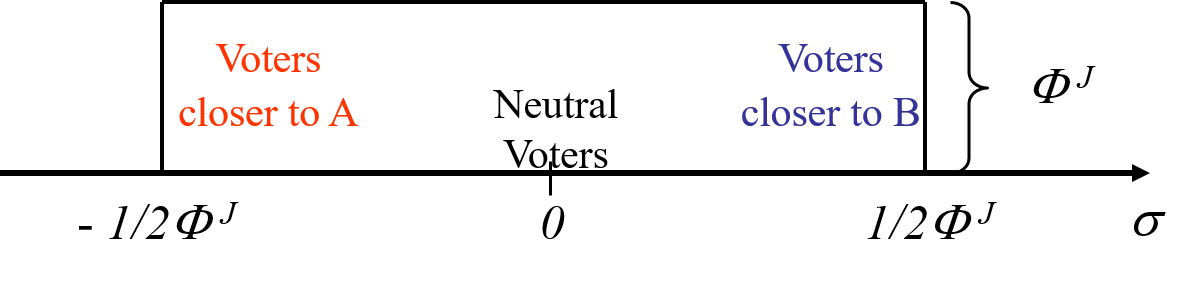
\includegraphics[scale=0.6]{ideologia1}
    \caption{Distribución de ideologías de votantes (en cada grupo)}
    \label{fig:baron1}
  \end{figure}
\end{frame}

\begin{frame}\frametitle{Votantes ``ideológicos'' (cont.)}
\begin{itemize}
\item Las decisiones de los votantes también están afectadas por la
  \textit{popularidad promedio de un candidato} antes de las
  elecciones $\longrightarrow$ los candidatos no pueden controlar esto
  [escándalo de emails Hillary Clinton; inundaciones en PBA efecto
  sobre Scioli]
  \item Entonces, $\delta>0$ implica que el candidato B es más popular
    y $\delta<0$ implica que el candidato A es más popular
\item Los candidatos solo pueden saber con qué probabilidad un
  escandalo puede ocurrir
  \end{itemize}
\end{frame}



\begin{frame}\frametitle{Votantes ``ideológicos'' (cont.)}
\begin{figure}[htbp]
    \centering 
    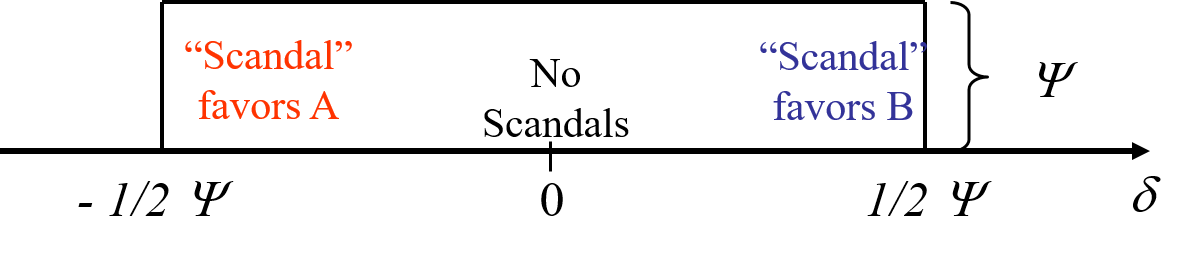
\includegraphics[scale=0.6]{ideologia2}
    \caption{Distribución de popularidad de candidatos}
    \label{fig:baron1}
  \end{figure}
\end{frame}



\begin{frame}\frametitle{Votantes ``ideológicos'' (cont.)}
\begin{itemize}
\item Entonces, los votantes consideran 3 (tres) elementos en base a
  los cuales decidir su voto: 1) posición de la política,
  $U^{J}(X_{A})$ y $U^{J}(X_{B})$; 2) ideología
  individual, $\sigma^{i,J}$; 3) popularidad promedio, $\delta$.
\item La predicción es que el votante ``i'' en el grupo ``J'' votará por el
  candidato B si:
  \begin{equation}
U^{J}(X_{B})+\sigma^{i,J}+\delta > U^{J}(X_{A})
    \end{equation}
\end{itemize}
\end{frame}


\begin{frame}\frametitle{Votantes ``ideológicos'': El votante swing}
\begin{itemize}
\item El votante swing es aquel que, una vez consideradas la
  plataforma de política y la popularidad del candidato, es
  \textit{indiferente} entres los candidatos A y B.
  \item ¿Por qué es este votante relevante? Porque un
    \textbf{pequeño} cambio en la plataforma de política de parte de
      un candidato hace que obtenga su voto.
      \item Notese que los candidatos anuncian sus plataformas antes
        que se conozca su popularidad promedio $\longrightarrow$ el
        candidato no sabe quien es el votante swing!
        \begin{equation}
\sigma^{J}=U^{J}(X_{B})-U^{J}(X_{A})-\delta
          \end{equation}
               \end{itemize}
\end{frame}



\begin{frame}\frametitle{Votantes ``ideológicos'' (cont.)}
\begin{figure}[htbp]
    \centering 
    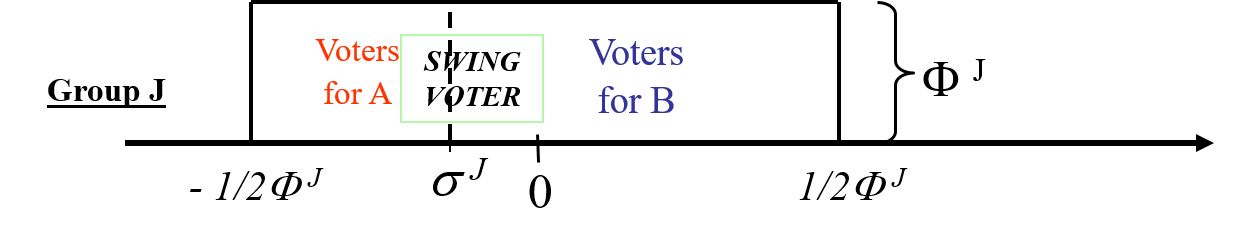
\includegraphics[scale=0.6]{ideologia3}
    \caption{La aparición del votante swing}
    \label{fig:baron1}
  \end{figure}
\end{frame}



\begin{frame}\frametitle{Votantes ``ideológicos'': Implicancias}
\begin{itemize}
\item Mas relevancia asignada al grupo más numeroso y al grupo menos
  ``ideologizado''
  \item Los candidatos pueden elegir la plataforma de política
    pensando en maximizar la probabilidad de ser electos sujetos a la
    eventualidad del escándalo $\longrightarrow$ como la probabilidad
    es uniforme, ambos incorporan eso
  \item Los candidatos terminan fijando las mismas plataformas
    \item Son relevantes aquellos votantes menos ideologizados (swing) $\longrightarrow$ faciles de
      convencer a través de la política
               \end{itemize}
\end{frame}






\end{document}


\section{Actores en el PFP}


 
      
  
 %  \begin{frame}\frametitle{Características de las PP: Volatilidad}
 %    \begin{itemize}
 %      \item Puede tomarse como una proxy de la evolución de la
 %        volatilidad en las políticas públicas el \textbf{índice de
 %          libertad económica} publicado por el Fraser Institute
 %        \item Puede verse en el gráfico que las políticas de Ecuador y
 %          Argentina tienden en promedio a ser más volátiles que las de
 %          Brasil y Colombia.
 %          \item Puede observase que en un período de más de 30 años,
 %            las oscilaciones de este indicador han sido más bruscas en
 %            Ecuador y Argentina que en Brasil y Colombia. Esto es en
 %            parte resultado de alta volatilidad de las políticas
 %            públicas. 
 %      \end{itemize}
 %    \end{frame}



    
 %    \begin{frame}\frametitle{Volatilidad de las políticas públicas}
 % \begin{figure}[htbp]\vspace{0cm}
 %    \centering
 %    \includegraphics[scale=0.35]{volatilidad1}
 %    \caption{Participación electoral en AL}
 %    \label{fig:1}
 %  \end{figure}
 %        \end{frame}

  
\end{document}
  